\documentclass[12pt]{article}

\textwidth=140mm
\textheight=245mm
\oddsidemargin=1truecm
\evensidemargin=1truecm
\voffset=-25mm


\usepackage{amsmath,amsfonts,amssymb,color,graphicx,overpic,} 
\usepackage{slashed}
\usepackage{epsfig}
%\documentstyle[12pt,epsfig]{article}
%\textwidth = 15.0cm
%\documentclass[12pt]{article}
\usepackage{amsmath}
\usepackage{ wasysym }
\usepackage{graphicx}
%\usepackage{fullpage}
\usepackage[english]{babel}
%\usepackage[top=2.0cm, bottom=2.0cm, left=2.0cm, right=2.0cm]{geometry}
\textheight = 24.8cm
\textwidth = 16.0cm
\hoffset = -0.6cm
%\let\savednewcommand\newcommand
  %\let\newcommand\renewcommand
  %\makeatletter
  %\input{size12.clo}
  %\makeatother
  %\let\newcommand\savednewcommand
%\voffset = -1.7cm
\voffset = -3.3cm
\usepackage{graphic x}
\usepackage{relsize}

\begin{document}

%\DeclareGraphicsExtensions{.png,.pdf}

\renewcommand{\arraystretch}{2}

\begin{titlepage}
\rightline{\large September 2014}
\vskip 2cm
\centerline{\Large \bf
Dissipative hidden sector dark matter}
%\vskip 0.5cm
%\centerline{\Large \bf two-component hidden sector dark matter model}

\vskip 2.2cm
\centerline{\large R.Foot\footnote{E-mail address: rfoot@unimelb.edu.au}, S.Vagnozzi\footnote{
E-mail address: svagnozzi@physics.unimelb.edu.au}}


\vskip 0.7cm
\centerline{\it ARC Centre of Excellence for Particle Physics at the Terascale,}
\centerline{\it School of Physics, University of Melbourne,}
\centerline{\it Victoria 3010 Australia}
\vskip 2cm
\noindent
%{\normalsize \bf Abstract} \newline \newline

A simple way of explaining dark matter without modifying known Standard Model physics is to require the existence of a hidden sector, which interacts with the visible one predominantly via gravity. We consider a hidden sector containing two stable particles charged under an unbroken $U(1) ^{'}$ gauge symmetry, hence featuring dissipative interactions. The massless gauge field associated with this symmetry can interact via kinetic mixing with the ordinary photon. In fact, such an interaction of strength $\epsilon \sim 10 ^{-9}$ appears to be necessary in order to explain galactic structure. We calculate the effect of this new physics on Big Bang Nucleosynthesis and its contribution to the relativistic energy density at Hydrogen recombination. Subsequently we examine the process of dark recombination, during which neutral dark states are formed, which is important for large-scale structure formation. We then analyze the phenomenology of our model in the context of galactic structure, and find that it can reproduce several observed features of spiral galaxies, including the cored density profile and the Tully-Fisher relation. Finally, we combine these analyses to set bounds on the parameter space of our model, which can serve as a guideline for future experimental searches.

 \end{titlepage}
 
 \newpage

\section{Introduction}

A variety of observations suggest the existence of non-baryonic dark matter in the Universe. Among these are measurements of the rotation curves of spiral galaxies, which are asymptotically flat \cite{rubin}. Dark matter is also required to explain the Cosmic Microwave Background (CMB) anisotropy spectrum (particularly the structure of the acoustic peaks), the matter power spectrum and large-scale structure (LSS) formation (see e.g. \cite{refregier}). Cosmological observations can be explained within the framework of the Friedmann-Robertson-Walker (FRW) model (see e.g. \cite{dodelson}), which assumes isotropy and homogeneity of the Universe on large scales. Comparison with observations require the total dark matter mass to be approximately five times that of baryonic matter.

The particle physics underlying dark matter is unknown but a promising possibility, widely discussed in recent literature (see e.g. \cite{feng,cline6,ringwald,broken}) is that dark matter resides in a hidden sector. That is, an additional sector containing particles and forces which interact with the known Standard Model particle content predominantly via gravity. A special case is mirror dark matter (MDM), where the hidden sector is exactly isomorphic to the Standard Model \cite{fundamentalimproper}. It has been shown that MDM can, under suitable assumptions and initial conditions, reproduce the successes of collisionless cold dark matter (CDM) on large scales, while deviating on small scales. This is important because such a model has the potential to address apparent shortcomings of collisionless CDM such as inferred cores in dark matter halos and the missing satellites problem \cite{berezhiani,mirrormattertype}.

Mirror dark matter is self-interacting due to an unbroken $U(1) ^{'}$ interaction (mirror electromagnetism). The associated gauge boson, the mirror photon, is massless, which implies that MDM is dissipative. Dissipative dark matter is a possible scenario, provided that there exists a substantial heat source that can replace the energy lost due to dissipative interactions. It has been argued \cite{spheroidal} that ordinary supernovae can provide such a heat source provided photon-mirror photon kinetic mixing exists. More in-depth studies of this possibility \cite{depth4} have shown that the model can reproduce several observational properties of spiral galaxies. MDM also seems to be capable of explaining the positive results from the direct detection experiments, especially the annual modulation signals observed by DAMA \cite{dama1} and CoGeNT \cite{cogent}, consistently with results from the other experiments \cite{dama,electronscattering}. For an up-to-date review and more detailed bibliography see \cite{review}.

It is possible that dark matter might arise from a more generic hidden sector with qualitatively similar features. So long as the hidden sector contains an unbroken $U(1) ^{'}$ gauge interaction, dissipative dark matter can arise. The simplest such generic hidden sector model contains two massive states, interacting with the $U(1) ^{'}$ gauge field (the \textit{dark photon}), with a priori unknown $U(1) ^{'}$ charges and masses. Such a model can then closely resemble MDM, with the lighter state corresponding to the mirror electron and the heavier state corresponding to mirror nuclei. Kinetic mixing can couple the massless $U(1) ^{'}$ gauge field with the ordinary photon. The physics is described by five free parameters. Our aim is to constrain this 5-dimensional parameter space using early Universe cosmology and galactic structure considerations.

The outline of this article, then, will be as follows. In Section 2 we define the model and examine some of its properties. Sections 3 and 4 will be devoted to studying its early Universe phenomenology, focusing in particular on how Big Bang Nucleosynthesis (BBN) and the onset of structure formation are affected. Section 5 is dedicated to analyzing the model in the context of galactic structure. Finally, in Section 6 we draw on the analyses of the previous sections to summarize the constraints on the model and in Section 7 we give some concluding remarks.

\section{Two-component hidden sector dark matter}

The model considered incorporates a hidden sector featuring an unbroken $U(1) ^{'}$ interaction. This means there is a massless gauge boson, called the \textit{dark photon} ($\gamma _{_D}$). The hidden sector will also contain two stable dark matter particles, $F_1$ and $F_2$, taken to be Dirac fermions, with masses $m _{F_1}$ and $m _{F_2}$. These two particles are assumed to be charged under the $U(1) ^{'}$ gauge group, with charges $Q _{F_1} ^{'}$ and $Q _{F_2} ^{'}$, opposite in sign but not necessarily the same in magnitude.

In the early Universe, the $U(1)'$ interactions would be expected to efficiently annihilate the symmetric component, meaning that the abundance of $F_1$ and $F_2$ dark matter is set by its particle-antiparticle asymmetry. This is an example of \textit{asymmetric} dark matter, which has been extensively discussed in recent literature \cite{reviewadm}. Dark matter asymmetry and local neutrality of the Universe then imply:
%
\begin{eqnarray}
n _{F_1}Q _{F_1} ^{'} + n _{F_2}Q _{F_2} ^{'} = 0 \ ,
\end{eqnarray}
%
where $n _{F_1}$ and $n _{F_2}$ are the number densities of $F _1$ and $F _2$ respectively. This is, of course, quite analogous to the situation with ordinary matter ($F_1 \sim$ electron, $F_2 \sim$ proton).

The only possible renormalizable and gauge-invariant mixing term that can be written is a kinetic mixing one \cite{foothe}, so the full Lagrangian of our model is:\footnote{Here and throughout the article, natural units with $\hbar = c = k _B = 1$ will be used.}
%
\begin{eqnarray}
{\cal L} = {\cal L} _{\text{SM}} -\frac{1}{4}F ^{'\mu \nu} F _{\mu \nu} ^{'} + \overline{F} _1(iD _{\mu}\gamma ^{\mu} - m _{F_1})F _1 + \overline{F} _2(iD _{\mu}\gamma ^{\mu} - m _{F_2})F _2 - \frac{\epsilon ^{'}}{2}F ^{\mu \nu} F _{\mu \nu} ^{'} \ ,
\end{eqnarray}
%
where $F _{\mu \nu} ^{'} = \partial _{\mu} A _{\nu} ^{'} - \partial _{\nu} A _{\mu} ^{'}$ is the field-strength tensor associated with the $U(1) ^{'}$ interaction, $A _{\mu} ^{'}$ being the relevant gauge field. The two dark fermions are described by the quantum fields $F_j$ and $D _{\mu}F _j = \partial _{\mu}F _j + ig ^{'}Q _{j} ^{'} A _{\mu} ^{'}F _j$, where $g ^{'}$ is the coupling constant relevant to this gauge interaction ($j=1,2$). The dark fermions are stable which is a consequence of the $U(1)'$
gauge symmetry and an accidental $U(1)$ global symmetriy  (implying conservation of $F_1$ and $F_2$ number). This is reminiscent of how $U(1)_Q$ and the accidental baryon number  symmetries arise in the Standard Model and how they stabilize the electron and proton. This is quite a general feature of hidden sector dark matter models and illustrates why they are so appealing theoretically: they typically predict a spectrum of massive, dark and stable particles.

The interactions of $F _1$ with the dark photon are characterized by the dark fine structure constant: $\alpha ^{'} \equiv (g'Q _{F_1}) ^2/4\pi$. The coupling of $F _2$ with the dark photon will be modified by the charge ratio: $Z' \equiv Q _{F_2} ^{'}/Q _{F_1} ^{'}$. By means of a non-orthogonal transformation, one can remove the kinetic mixing and show that the net effect of the relevant term is to provide the dark fermions with a tiny ordinary electric charge \cite{holdom}. The physical photon now couples to dark fermions with charge:
%
\begin{eqnarray}
g'Q _{F_j} ^{'} \epsilon ^{'} \equiv \epsilon _{F_j}e \ .
\end{eqnarray}
%
Thus the fundamental physics of the model is described by 5 parameters: $m _{F_1},m _{F_2},\alpha ^{'},Z ^{'}$ and $\epsilon \equiv \epsilon _{F_1}$ (note that $\epsilon _{F_2} = Z ^{'}\epsilon _{F_1}$, and is therefore not an independent parameter). For definiteness we will focus on the case $m _{F_1} \ll m _{F_2}$, with $Z ^{'}$ being an integer.

Clearly it is entirely possible for our model to be the low energy effective field theory limit of a more complex theory. In this context, $F _1$ and/or $F _2$ might represent bound states (dark nuclei), which could be bound together by some interaction which resembles the strong one. In this case, the $F_1$/$F_2$ masses arise from a dark confinement scale (analogous to $\Lambda _{\text{QCD}}$ in the Standard Model) rather than being a bare mass term. Alternatively, the mass terms for $F _j$ might originate from a hidden sector scalar, $S$, by means of a Lagrangian term of the form $\lambda _jS\bar{F} _jF _j$, with $\langle S \rangle \neq 0$.

Some possible implications of this model for dark matter direct detection experiments have been discussed previously in \cite{hiddensector}. Furthermore, as explained in the introduction, the dark matter phenomenology is similar but generalizes the MDM case. Related hidden sector models, featuring an unbroken $U(1) ^{'}$ interaction, have also been discussed in recent literature, e.g. \cite{feng,cline6,petrakiatomic} and much earlier in \cite{goldberghall}. However, these models assume parameter space where the dark matter galactic halo is in the form of atoms (or a non dissipative plasma), and thus can be collisional but generally not dissipative.\footnote{An alternative possibility examined in recent literature, known as Double-Disk Dark Matter (DDDM), explores the scenario where only a subdominant component of the dark matter exhibits dissipative interactions \cite{dddm}. These dissipative dynamics allow for DDDM to cool efficiently and form a thin dark matter disk, similar to the baryonic disk.} We consider the case where the galactic halo is in the form of a roughly spherical dissipative plasma. Such a spherical plasma would cool via dissipative processes, for instance dark bremsstrahlung, unless a substantial heat source exists. Here a pivotal role is played by the kinetic mixing interaction: kinetic mixing induced processes within the core of ordinary supernovae (dominated by plasmon decay \cite{raf,updated}) are presumed to provide the heat source that replaces the energy lost to dissipative interactions. This is possible provided $\epsilon \sim 10 ^{-9}$ and $m _{F_1} \lesssim {\rm few} \times T _{\text{SN}} \simeq 100 \ {\rm MeV}$, where $T _{\text{SN}}$ is the temperature reached in the core of ordinary supernovae.\footnote{Although the kinetic mixing parameter is very small, $\epsilon \sim 10 ^{-9}$, this does not represent a theoretical problem, such as radiative instability. Indeed, as discussed in \cite{poincare}, small values for the coupling are technically natural (in the sense of 't Hooft) since, in the limit $\epsilon \rightarrow 0$, an enhanced Poincar\'e symmetry arises: ${\cal G} _P ^{\text{SM}} \otimes {\cal G} _P ^{\text{HS}}$, where ${\cal G} _P$ denotes the Poincar\'e group and SM and HS stand for Standard Model and Hidden Sector respectively.} A lower limit $m _{F_1} \gtrsim 0.01 \ {\rm MeV}$ arises from studies of Red Giants \cite{redgiants} and White Dwarfs \cite{whitedwarfs,updated} (see \cite{bailey} for a summary of relevant bounds).

Finally, one can also consider a two-component hidden sector model where the two dark matter particles are bosons rather than fermions, charged under an $U(1)'$ interaction. In the case of two scalar particles, $B _j$, the Lagrangian is:
%
\begin{eqnarray}
{\cal L} = {\cal L} _{\text{SM}} - \frac{1}{4}F ^{'\mu \nu}F ^{'} _{\mu \nu} + \left ( D _{\mu}B _j \right ) ^{\dagger}\left ( D ^{\mu}B _j \right ) - m _{B _j} ^2B _j ^{\dagger}B _j - \frac{\epsilon ^{'} _B}{2}F ^{\mu \nu} F _{\mu \nu} ^{'} \ ,
\label{bosonic}
\end{eqnarray}
%
where $j=1,2$ (with summation over $j$ implied). As in the two-component fermion case, one can consider the general case where the $U(1)'$ charges of $B _1$ and $B _2$ are different, with $Z' _B$ being the charge ratio. As before, the Lagrangian in Eq.(\ref{bosonic}) possesses two accidental $U(1)$ symmetries which imply conservation of $B _1$ and $B _2$ number, and hence stability of the dark matter particles. Again, the kinetic mixing term will play a dominant role in the cosmological and galactical dynamics of such a model. Barring factors of order unity to account for spin statistics, the analysis we will perform in the following sections will hold for this bosonic model as well as the fermionic one. In particular, the bounds that are summarized in Section 6 hold for the bosonic case, up to factors of order unity. For definiteness, though, we will focus on the fermionic model.

\section{Cosmology of the early Universe}

\subsection{Evolution of $\frac{T _{\gamma _{_D}}}{T _{\gamma}}$}

Successful cosmology, BBN and LSS strongly constrain exotic contributions to the energy density during the radiation dominated era. If we define $T _{\gamma}$[$T _{\gamma _{_D}}$] and $T _{\nu}$ to be the photon [dark photon] and neutrino temperatures, then we require $T _{\gamma _{_D}} \ll T _{\gamma}$ (the exact mechanism that provides such an initial condition will not be of our concern, although asymmetric reheating is possible within inflationary models \cite{hodges}).\footnote{We only require $T _{\gamma _{_D}} \ll T _{\gamma}$ at, say, the QCD phase transition, $T _{\text{QCD}} \sim 100$ MeV. Thus, even if the Universe started with $T _{\gamma _{_D}} = T _{\gamma}$ at $T > T _{\text{QCD}}$, the heating of the ordinary sector at the QCD phase transition would be sufficient to establish the necessary initial condition, $T _{\gamma _{_D}} \ll T _{\gamma}$, at $T _{\text{QCD}}$.} As discussed previously, kinetic mixing confers a tiny ordinary electric charge to dark fermions. It follows that in the early Universe energy and entropy can be transferred between the sectors. Thus even if the Universe starts with $T _{\gamma _{_D}}/T _{\gamma}=0$, $T _{\gamma _{_D}}$ will be generated as entropy is transferred from the visible to the hidden sector. In the following work we first study the evolution of $T _{\gamma _{_D}}/T _{\gamma}$ (with initial condition $T _{\gamma _{_D}}/T _{\gamma} = 0$), and then consider the relevant cosmological constraints.

In the early Universe energy is transferred between the sectors via various processes, including (to order $\epsilon ^2$) $e \overline{e} \rightarrow F _1 \overline{F} _1$, $eF_1 \rightarrow eF_1$, $e \overline{e} \rightarrow F _2 \overline{F} _2$, $\gamma F_1 \rightarrow \gamma _{_D}F _1$, and so on. Processes involving $F_2$ can be approximately neglected if $F_2$ is much heavier than $F_1$ [simple analytic calculations indicate that for $m _{F_2} \gg {Z'} ^2\max (m _e , m _{F_1})$ the energy transfer between the sectors is dominated by $F_1$ production]. Of the remaining processes, $e \overline{e} \rightarrow F _1 \overline{F} _1$ is expected to dominate (for $T _{\gamma} \gtrsim m _e$), given that the rates of all other two-body processes are smaller by a factor of $\lesssim n _{F_1}/n _e \sim (T _{\gamma _{_D}}/T _{\gamma}) ^3$, and typically we are constrained to reside in the region of parameter space where $(T _{\gamma _{_D}}/T _{\gamma}) ^3 \ll 1$. Hence for $m _{F_1} \gtrsim 0.1 \ {\rm MeV}$, we consider just one production process, $e\overline{e} \rightarrow F_1\overline{F}_1$.\footnote{While this work was in progress, the paper \cite{redondo} appeared which considered $N_{\text{eff}}$ constraints on a related model. There they considered additional production channels, such as $\gamma F_1 \rightarrow \gamma_{_D} F_1$, for a wide range of parameter space. The effect of these extra channels is to tighten constraints on epsilon by around a factor of 2.}

For $m _{F_1} \lesssim 0.1$ MeV, one could consider  processes such as $\gamma F _1 \rightarrow \gamma _{_D}F _1$ in addition to $e\overline{e} \rightarrow F _1\overline{F} _1$. Although the rate for $\gamma F_1 \rightarrow \gamma _{_D}F _1$ is suppressed relative to $e\overline{e} \rightarrow F_1 \overline{F} _1$ by $\sim \left ( T _{\gamma _{_D}}/T _{\gamma} \right ) ^3$ for $T _{\gamma} \gtrsim m _e$, for $T _{\gamma} \lesssim m _e$ the rate of $\gamma F_1 \rightarrow \gamma _{_D}F _1$ can become important and eventually dominate.\footnote{Another $F_1$ production channel that could be relevant for very low $F_1$ mass is plasmon decay ($\gamma \rightarrow F _1\overline{F} _1$). It can become important when $m _{F_1} \lesssim \omega _P/2$, where $\omega _P = \sqrt{4\pi\alpha T ^2/9}$ is the plasma frequency (see e.g. \cite{updated}). This implies that during the period of interest (from BBN to the formation of the CMB) plasmon decay is only important for $m _{F_1} \lesssim 50 \ {\rm keV}$.} Here we shall focus on $m _{F_1} \gtrsim 0.1$ MeV, where $e\overline{e} \rightarrow F _1\overline{F} _1$ is the dominant process affecting the evolution of the temperatures. Thus, our analysis will only be strictly valid in the range $0.1 \ {\rm MeV} \lesssim m _{F_1} \lesssim 100 \ {\rm MeV}$, while the study of the region $0.01 \ {\rm MeV} \lesssim m _{F_1} \lesssim 0.1 \ {\rm MeV}$ will require further work. Restricting ourselves to the region of parameter space $m _{F_1} \gtrsim 0.1 \ {\rm MeV}$ also bypasses several other complications which arise in the context of galactic structure (Section 5).


The cross-section for $e \overline{e} \rightarrow F_1 \overline{F}_1$ is analogous to that of muon pair-production, with the essential difference being that the coupling of $F_1$ to the ordinary photon is now given by $\epsilon e$. The cross-section for this process is:
%
\begin{eqnarray}
\sigma = \frac{4\pi}{3s^3} \epsilon ^2 \alpha ^2 \sqrt{\frac{s^2 - 4 m _{F_1} ^2}{s^2 - 4 m _{e} ^2}} \left (s^2 + 2 \left (m _{e} ^2 + m _{F_1} ^2 \right )s + 4m _{e} ^2 m _{F_1} ^2 \right ) \ ,
\end{eqnarray}
%
where $\sqrt{s}$ is the centre-of-momentum energy of the system, $\alpha = e^2/4\pi$ is the fine-structure constant and $m _{e}$ is the electron mass. The following treatment generalizes the MDM case analyzed in \cite{predictions}, which itself followed earlier works \cite{updated,carlson,ciarcellutiliege}. Energy is transferred between the visible and dark sectors within a co-moving volume $R^3$ ($R$ being the scale factor) at a rate given by:
%
\begin{eqnarray}
\frac{dQ}{dt} = R^3 n _{e} n _{\overline{e}} \langle \sigma v_{\text{M\o l}} {\cal E} \rangle \ ,
\label{dqdt}
\end{eqnarray}
%
where $\langle \sigma v_{\text{M\o l}} \rangle$ is the thermally averaged cross-section, $ v_{\text{M\o l}}$ is the M$\o$ller velocity and ${\cal E} = E_1 + E_2$ is the total energy of the system. Following \cite{ciarcellutiliege,gondologelmini}, we replace the exact Fermi-Dirac distribution with the simpler Maxwellian one, so that the thermally averaged cross-section is given by:
%
\begin{eqnarray}
\langle \sigma v_{\text{M\o l}} {\cal E} \rangle = \frac{\mathlarger \int d^3p_1 d^3p_2 \ e^{-\frac{E_1}{T}} e^{-\frac{E_2}{T}} \ \sigma v_{\text{M\o l}}{\cal E}}{\mathlarger \int d^3p_1 d^3p_2 \ e^{-\frac{E_1}{T}}e^{-\frac{E_2}{T}}} \ .
\end{eqnarray}
%
To evaluate the thermally averaged cross-section, similar steps as in \cite{ciarcellutiliege,gondologelmini} can be followed, yielding:
%
\begin{eqnarray}
\langle \sigma v_{\text{M\o l}}{\cal E} \rangle = 
\frac{\omega}{8m_e^4 T_{\gamma}^2 {[K_2(\frac{m_e}{T_{\gamma}})]}^2}
\mathlarger \int _{4{\cal M}^2}^{\infty} ds \ \sigma (s - 4m_e^2)
\sqrt{s} \mathlarger \int _{\sqrt{s}}^{\infty} dE_+ \ e^{-\frac{E_+}{T _{\gamma}}} E_+ \sqrt{\frac{E _+ ^2}{s} - 1} \ ,
\label{sig}
\end{eqnarray}
%
where $\omega \approx 0.8$ takes into account various approximations such as the aforementioned use of a Maxwell-Boltzmann distribution in lieu of the actual Fermi-Dirac one in evaluating the thermally averaged cross-section \cite{ciarcellutiliege}. $K_2(z)$ is the modified Bessel function of the second kind and argument $z$, and ${\cal M} \equiv \max(m _e, m _{F_1})$. Finally, we can write (see for instance \cite{earlyuniverse}):
%
\begin{eqnarray}
n _{e} \simeq n _{\overline{e}} = \frac{1}{\pi ^2} \int _{m_e} ^{\infty} dE \ \frac{\sqrt{E^2 - m _e ^2}E}{1 + e^{\frac{E}{T _{\gamma}}}} \ .
\end{eqnarray}
%

Since self-interaction rates are bigger than the rates of kinetic mixing induced processes by many orders of magnitude ($\sim 1/\epsilon ^2$), the overall system can be modelled as being composed of two subsystems, one at temperature $T _{\gamma}$ and the other at temperature $T _{\gamma _{_D}}$, exchanging energy while remaining instantaneously in thermodynamical equilibrium. This system is somewhat analogous to that of a block of ice melting in a glass of water (e.g. \cite{feynman}). The second law of thermodynamics can therefore be applied to it. In principle, the neutrino subsystem should be taken into account too. In practice the net transfer of energy to the neutrino subsystem can be neglected since energy transfer to the dark sector happens predominantly after neutrino kinetic decoupling. This means that $dS _{\nu} \simeq 0$. Nevertheless, the evolution of $T _{\nu}$ will still have to be taken into account, though it trivially scales as the inverse of the scale factor (see e.g. \cite{earlyuniverse}).

The second law of thermodynamics states that the change in entropy in the visible sector is given by:
%
\begin{eqnarray}
dS = -\frac{dQ}{T _{\gamma}} \ .
\label{entropyordinary}
\end{eqnarray}
%
Similarly, the change in entropy for the dark sector is:
%
\begin{eqnarray}
dS ^{'} = \frac{dQ}{T _{\gamma _{_D}}} \ .
\label{entropydark}
\end{eqnarray}
%
An useful way to express the entropy of a particle species in cosmology is given in e.g. \cite{earlyuniverse}:
%
\begin{eqnarray}
S = \frac{\rho + p}{T}R^3 \ ,
\label{entropycosmology}
\end{eqnarray}
%
where $\rho$, $p$ and $T$ denote its energy density, pressure and temperature respectively. Taking the derivative with respect to time on both sides of Eqs.(\ref{entropyordinary},\ref{entropydark}) and combining the result with Eqs.(\ref{dqdt},\ref{entropycosmology}) yields:
%
\begin{eqnarray}
\frac{d}{dt} \left [ \frac{(\rho _{\gamma} + p _{\gamma} + \rho _e + p _e)R^3}{T _{\gamma}}\right ] &=& - \frac{n _e n _{\overline{e}} \langle \sigma v_{M\o l} {\cal E} \rangle R^3}{T _{\gamma}} \ , \nonumber \\
\frac{d}{dt} \left [ \frac{(\rho _{\gamma _{_D}} + p _{\gamma _{_D}} + \rho _{F_1} + p _{F_1})R^3}{T _{\gamma _{_D}}}\right ] &=& \frac{n _e n _{\overline{e}} \langle \sigma v_{M\o l} {\cal E} \rangle R^3}{T _{\gamma _{_D}}} \ ,
\label{entropy1}
\end{eqnarray}
%
where we have neglected the neutrino contribution to the entropy change, which is justified as $dS _{\nu} \simeq 0$, as discussed above. In Eqs.(\ref{entropy1}) and below, we have defined $\rho _e \equiv \rho _e + \rho _{\bar{e}}$, and similarly for $p _e$, $\rho _{F_1}$ and $p _{F_1}$.

The $^{00}$ component of the Einstein field equations for the FRW metric describes the evolution of the scale factor $R$. This is known as first Friedmann equation, and in a flat Universe takes the form:
%
\begin{eqnarray}
\left ( \frac{\dot{R}}{R} \right ) ^2 = \frac{8\pi G_N}{3} \left [\rho _{\gamma} + \rho _e + \rho _{\nu} + \rho _{\gamma _{_D}} + \rho _{F_1} \right ] \ .
\label{Friedmann}
\end{eqnarray}
%
Defining $x \equiv m _e/T _{\gamma}$, energy densities and pressures in the visible sector are given in e.g. \cite{earlyuniverse}:
%
\begin{eqnarray}
\rho _{\gamma} &=& \frac{\pi ^2}{15} T _{\gamma} ^4 \ , \nonumber \\
p _{\gamma} &=& \frac{\pi ^2}{45} T _{\gamma} ^4 \ , \nonumber \\
\rho _e &=& \frac{2T _{\gamma} ^4}{\pi ^2} \mathlarger \int _{x} ^{\infty}du \ \frac{(u^2 - x^2)^{\frac{1}{2}}u^2}{1 + e^u} \ , \nonumber \\
p _e &=& \frac{2T _{\gamma} ^4}{3\pi ^2} \mathlarger \int _{x} ^{\infty}du \ \frac{(u^2 - x^2)^{\frac{3}{2}}}{1 + e^u} \ , \nonumber \\
\rho _{\nu} &=& \frac{7\pi ^2}{40} T _{\nu} ^4 \ .
\end{eqnarray}
%
Similarly for the dark sector, with $x ^{'} \equiv m _{F_1}/T _{\gamma _{_D}}$:
%
\begin{eqnarray}
\rho _{\gamma _{_D}} &=& \frac{\pi ^2}{15} {T _{\gamma _{_D}}}^4 \ , \nonumber \\
p _{\gamma _{_D}} &=& \frac{\pi ^2}{45} {T _{\gamma _{_D}}} ^4 \ , \nonumber \\
\rho _{F_1} &=& \frac{2{T _{\gamma _{_D}}} ^4}{\pi ^2} \mathlarger \int _{x'} ^{\infty}du \ \frac{(u^2 - {x'}^2)^{\frac{1}{2}}u^2}{1 + e^u} \ , \nonumber \\
p _{F_1} &=& \frac{2{T _{\gamma _{_D}}} ^4}{3\pi ^2} \mathlarger \int _{x'} ^{\infty}du \ \frac{(u^2 - {x'}^2)^{\frac{3}{2}}}{1 + e^u} \ .
\end{eqnarray}
%

Considering the neutrino subsystem, the neutrino temperature scales as $T _{\nu} \propto 1/R$ which follows from $dS _{\nu} \simeq 0$. Noting that all proportionality factors cancel [being there the same power of the scale factor $R$ on both sides of Eqs.(\ref{entropy1})], $R$ in Eqs.(\ref{entropy1}) can effectively be replaced by $1/T _{\nu}$. Accordingly, Eqs.(\ref{entropy1}) can be expressed as:
%
\begin{eqnarray}
\frac{d}{dt} \left [ \frac{(\rho _{\gamma} + p _{\gamma} + \rho _e + p _e)}{T _{\gamma} T _{\nu} ^3}\right ] &=& - \frac{n _e n _{\overline{e}} \langle \sigma v_{M\o l} {\cal E} \rangle }{T _{\gamma} T _{\nu} ^3} \ , \nonumber \\
\frac{d}{dt} \left [ \frac{(\rho _{\gamma _{_D}} + p _{\gamma _{_D}} + \rho _{F_1} + p _{F_1})}{T _{\gamma _{_D}}T _{\nu} ^3}\right ] &=& \frac{n _e n _{\overline{e}} \langle \sigma v_{M\o l} {\cal E} \rangle }{T _{\gamma _{_D}}T _{\nu} ^3} \ ,
\label{system1}
\end{eqnarray}
%
and Eq.(\ref{Friedmann}) as:
%
\begin{eqnarray}
\frac{1}{T _{\nu}} \frac{dT _{\nu}}{dt} &=& - \sqrt{\frac{8\pi G_N}{3} \left ( \rho _{\gamma} + \rho _e + \rho _{\nu} + \rho _{\gamma _{_D}} + \rho _{F_1} \right )} \ .
\label{friedmannbis}
\end{eqnarray}
%
Some manipulation shows that Eqs.(\ref{system1}) can be brought to the form:
%
\begin{eqnarray}
\zeta \frac{dT _{\gamma}}{dt} + \kappa \frac{dT _{\nu}}{dt} &=& - \frac{n _{e} n _{\overline{e}} \langle \sigma v _{M\o l} {\cal E} \rangle }{T _{\gamma} ^3} \ , \nonumber \\
\zeta ^{'} \frac{dT _{\gamma _{_D}}}{dt} + \kappa ^{'} \frac{dT _{\nu}}{dt} &=& \frac{n _{e} n _{\overline{e}} \langle \sigma v _{M\o l} {\cal E} \rangle }{T _{\gamma _{_D}} ^3} \ ,
\label{sistema1}
\end{eqnarray}
%
where:
%
\begin{eqnarray}
\zeta & \equiv &  \frac{3\rho _{\gamma}}{T _{\gamma} ^4} + \frac{3p _{\gamma}}{T _{\gamma} ^4} + \frac{3\rho _e}{T _{\gamma} ^4} + \frac{3p _e}{T _{\gamma} ^4} + \frac{2m _{e} ^2}{\pi ^2 T _{\gamma} ^2} \int _{x} ^{\infty} du \ \frac{(u^2 - x^2)^{-\frac{1}{2}} u^2 + (u^2 - x^2)^{\frac{1}{2}}}{1 + e^u} \ , \nonumber \\
\kappa & \equiv & - \left ( \frac{3\rho _{\gamma}}{T _{\gamma} ^3} + \frac{3p _{\gamma}}{T _{\gamma} ^3} + \frac{3\rho _e}{T _{\gamma} ^3} + \frac{3p _e}{T _{\gamma} ^3} \right ) \frac{1}{T _{\nu}} \ , \nonumber \\
\zeta ^{'} & \equiv & \frac{3\rho _{\gamma _{_D}}}{{T _{\gamma _{_D}}} ^4} + \frac{3p _{\gamma _{_D}}}{{T _{\gamma _{_D}}}^4} + \frac{3\rho _{F_1}}{{T _{\gamma _{_D}}} ^4} + \frac{3p _{F_1}}{{T _{\gamma _{_D}}} ^4} + \frac{2m _{F_1} ^2}{\pi ^2 {T _{\gamma _{_D}}} ^2} \int _{x'} ^{\infty} du \ \frac{(u^2 - {x'}^2)^{-\frac{1}{2}} u^2 + (u^2 - {x'}^2)^{\frac{1}{2}}}{1 + e^u} \ , \nonumber \\
\kappa ^{'} & \equiv & - \left ( \frac{3\rho _{\gamma _{_D}}}{{T _{\gamma _{_D}}}^3} + \frac{3p _{\gamma _{_D}}}{{T _{\gamma _{_D}}} ^3} + \frac{3\rho _{F_1}}{{T _{\gamma _{_D}}} ^3} + \frac{3p _{F_1}}{{T _{\gamma _{_D}}} ^3} \right ) \frac{1}{T _{\nu}} \ .
\label{sistemo}
\end{eqnarray}
%

We are now left with a closed system of three differential equations [Eqs.(\ref{friedmannbis},\ref{sistema1})] for three unknowns ($T _{\gamma}$, $T _{\gamma _{_D}}$ and $T _{\nu}$). Given suitable initial conditions, then, the system can be solved numerically to give the evolution of these three quantities. An example is presented in Figure \ref{fig:evolution of x}, where the evolution of $T _{\gamma _{_D}}/T _{\gamma}$ is plotted as a function of $T _{\gamma}$ for different values of $m _{F_1}$ and for $\epsilon = 10 ^{-9}$. Note that the flow of time is from the right to the left.

\begin{figure}[htpb]
    \centering
        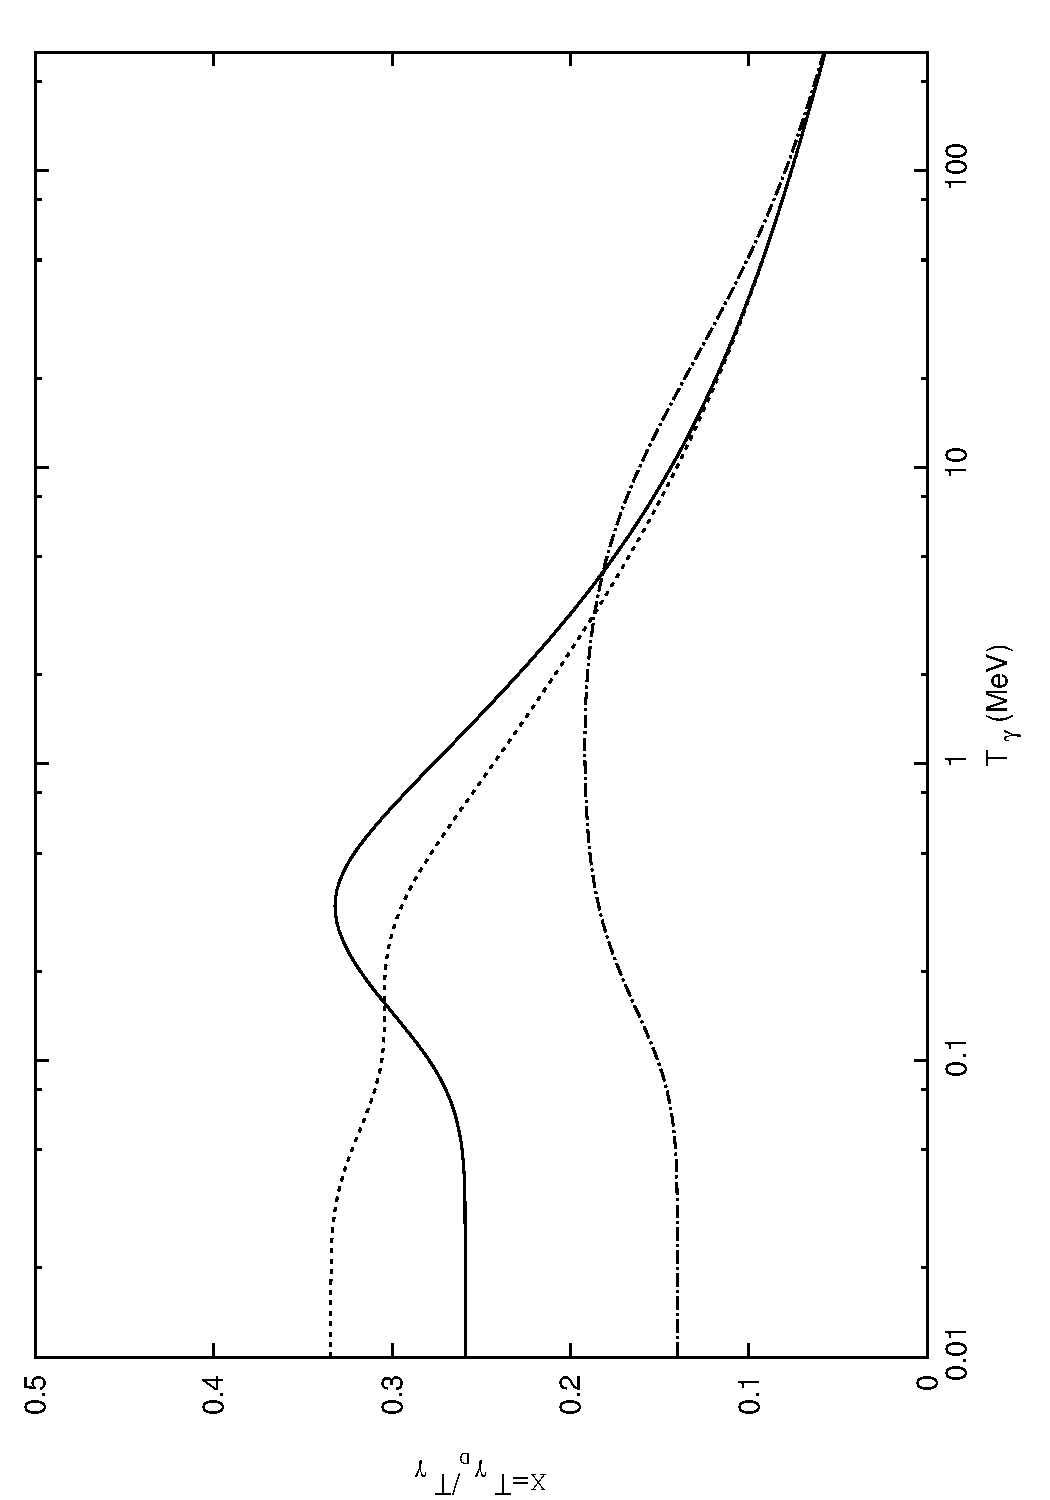
\includegraphics[scale=0.5, angle=270]{fig1quater_9}
 %       \rule{35em}{0.5pt}
    \caption{Evolution of ${\cal X} \equiv T _{\gamma _{_D}}/T _{\gamma}$ for $m_{F_1}=10$ MeV (dot-dashed line), $m_{F_1}=1$ MeV (solid line) and $m_{F_1}=0.1$ MeV (dashed line).}
    \label{fig:evolution of x}
\vskip 0.8cm
\end{figure}

%\vskip 1.4 cm

It can be seen from Figure \ref{fig:evolution of x} that $T _{\gamma _{_D}}/T _{\gamma}$ asymptotically approaches a constant at late times. We would like to find an approximate analytic expression for the asymptotic value of $T _{\gamma _{_D}}/T _{\gamma}$. It is perhaps useful to recall the results obtained for MDM. In this context, MDM can be viewed as a special case of our model in the limit where $m _{F_1} = m _e$. For the case of MDM it has been found that $T _{{\gamma} ^{'}}/T _{\gamma}$ (where $\gamma ^{'}$ denotes the mirror photon, which is of course analogous to our dark photon, $\gamma _{_D}$) asymptotically evolves to \cite{predictions}:
%
\begin{eqnarray}
\frac{T _{{\gamma} ^{'}}}{T _{\gamma}} \simeq 0.31 \left ( \frac{\epsilon}{10^{-9}} \right ) ^{\frac{1}{2}} \ .
\label{xmirror}
\end{eqnarray}
%
More generally, $m _{F_1} \neq m _e$ in the context of our two-component hidden sector model, and one expects a somewhat different behavior in $T _{\gamma _{_D}}/T _{\gamma}$ to account for this $m _{F_1}$ dependence. Previous work in the MDM context shows that in the limit of $T _{\gamma} \gg m _e$, an analytic expression can be found for $T _{{\gamma} ^{'}}/T _{\gamma}$ \cite{ciarcellutiliege}:
%
\begin{eqnarray}
\frac{T _{{\gamma} ^{'}}}{T _{\gamma}} \propto \sqrt{\epsilon} \left [ \frac{1}{T} - \frac{1}{T_i} \right ] ^{\frac{1}{4}} \ ,
\label{epsilont}
\end{eqnarray}
%
with an assumed initial condition $T _{{\gamma} ^{'}} = 0$ at $T _{\gamma} = T_i$. For $T _{\gamma} \sim m _e$, energy transfer to the mirror sector cuts off, as the process $e\overline{e} \rightarrow e ^{'}\overline{e} ^{'}$ becomes infrequent due to Boltzmann suppression of $e$, $\overline{e}$ number densities.

We can attempt to generalize the result to our case. The process $e\overline{e} \rightarrow F _1\overline{F} _1$ will cease to be important at temperatures below $\sim {\cal M} \equiv \max (m _e , m _{F_1})$. Eq.(\ref{epsilont}) then suggests that the asymptotic value of the ratio $T _{\gamma _{_D}}/T _{\gamma}$ is proportional to $\sqrt{\epsilon} \left (m _e/{\cal M} \right ) ^{\frac{1}{4}}$. This intuition has been verified numerically, by evolving for different values of $\epsilon$ and $m _{F_1}$. Numerically, we find that the asymptotic value of $T _{\gamma _{_D}}/T _{\gamma}$ can be expressed in the form:
%
\begin{eqnarray}
\frac{T _{\gamma _{_D}}}{T _{\gamma}} & \simeq & 0.31 \sqrt{\frac{\epsilon}{10^{-9}}} \left (\frac{m _e}{{\cal M}} \right ) ^{\frac{1}{4}} \ , \nonumber \\
{\cal M} & \equiv & \max (m _e, m _{F_1}) \ ,
\label{masterformula}
\end{eqnarray}
%
for parameters in the range $\epsilon \sim 10 ^{-9}$ and $0.1$ MeV $\lesssim m _{F_1} \lesssim 100$ MeV.

One can also attempt to understand the shape of the curves in Figure \ref{fig:evolution of x}. At early times ($T _{\gamma} \gg m _{F_1},m _e$) the curves overlap, following a $T _{\gamma _{_D}}/T _{\gamma} \propto \left (1/T _{\gamma} \right ) ^{\frac{1}{4}}$ behavior consistent with the analytic solution previously discussed. At some later time corresponding to $T _{\gamma} \sim {\cal M}$, the curves start deviating from the analytic solution. The rising of the various curves at different temperatures and with characteristic bumps can be understood in terms of annihilation processes which are heating the respective sectors roughly at the temperature corresponding to the mass of the particle-antiparticle pair which is annihilating. That is, electron-positron and $F _1$-$\overline{F} _1$ annihilations explain the deviation of the numerical solution from the simpler analytic one. Once the annihilation processes are over, $T _{\gamma _{_D}}/T _{\gamma}$ reaches its asymptotic value.

\subsection{Calculation of $\delta N _{\text{eff}}$[CMB]}

We now compute the modification of the energy density at the Hydrogen recombination epoch in the early Universe. A way to parametrize this extra energy density is in terms of an effective number of neutrino species. Recall that the relativistic energy density component at recombination can be expressed as:
%
\begin{eqnarray}
\rho _{\text{rad}} = \left (1 + \frac{7}{8} \left (\frac{4}{11} \right) ^{\frac{4}{3}} N _{\text{eff}}[\text{CMB}] \right ) \rho _{\gamma} \ ,
\end{eqnarray}
%
where the factor of $7/8$ takes into account the different statistical nature (fermionic instead of bosonic) of neutrinos with respect to photons, and the factor of $4/11$ takes care of $\gamma$ heating due to $e \overline{e}$ annihilation after neutrino kinetic decoupling (see for instance \cite{earlyuniverse}). $N _{\text{eff}}$ is referred to as the effective number of neutrinos, and is predicted to be $N _{\text{eff}} \simeq 3.046$ in the Standard Model (see e.g. \cite{mangano}). Observations from WMAP \cite{wmapx}, the South Pole Telescope \cite{sptx}, the Atacama Cosmology Telescope \cite{atax} and the Planck mission \cite{plax} are consistent with the Standard Model predictions and can be used to constrain $\delta N _{\text{eff}}[\text{CMB}] \equiv N _{\text{eff}}[\text{CMB}] - 3.046$. A 2$\sigma$ upper limit on $\delta N _{\text{eff}}$[CMB] is indicatively $\delta N _{\text{eff}}[\text{CMB}] < 0.84$. Note we can write:
%
\begin{eqnarray}
\delta N _{\text{eff}}[\text{CMB}] = 3 \left (\left [\frac{T _{\nu} ( \epsilon )}{T _{\nu} ( \epsilon = 0)}\right ]^4 - 1 \right ) + \frac{8}{7} \left ( \frac{T _{\gamma _{_D}} ( \epsilon )}{T _{\nu} ( \epsilon = 0)} \right )^4 \ ,
\label{Neffcmb}
\end{eqnarray}
%
where the temperatures are evaluated at photon decoupling, $T _{\gamma} \simeq 0.26$ eV. The two terms on the right-hand side of Eq.(\ref{Neffcmb}) account for distinct effects. Firstly, the process $e \overline{e} \rightarrow F_1 \overline{F}_1$ will increase $T _{\gamma _{_D}}$ at the expense of $T _{\gamma}$, thus reducing $T _{\gamma}/T _{\nu}$ and effectively increasing the number of neutrino species at recombination. The second term is the direct increase in $N _{\text{eff}}[\text{CMB}]$ due to the increase in $T _{\gamma _{_D}}$ itself.

One has to pay attention when using $\delta N _{\text{eff}}$[CMB] to set constraints on the parameter space, since the addition of energy density is not the only effect to consider. Prior to recombination of $F _1$ and $F _2$ into neutral dark states, dark matter behaves like a tightly coupled fluid, analogous to the photon-baryon fluid in the visible sector. This fluid undergoes acoustic oscillations, which suppress power on small scales, hence behaving very differently from collisionless CDM. Thus, there are two quite different possible effects for the CMB to consider. The first is the extra energy density as parametrized by $\delta N _{\text{eff}}$[CMB], and the second is the effect of dark acoustic oscillations prior to dark recombination. In this section we consider the energy density modification, while the constraints arising from dark acoustic oscillations will be dealt with in Section 4.

%Observe that as $m _{F_1}$ drops below $m _e$, the rate for the process $e\overline{e} \rightarrow F _1\overline{F} _1$ becomes approximately independent of $m _{F_1}$. In principle, for $m _{F_1} \lesssim 0.1$ MeV, one could consider the process $\gamma F _1 \rightarrow \gamma _{_D}F _1$ in addition to $e\overline{e} \rightarrow F _1\overline{F} _1$. Although the rate for $\gamma F_1 \rightarrow \gamma _{_D}F _1$ is suppressed relative to $e\overline{e} \rightarrow F_1 \overline{F} _1$ by $\sim \left ( T _{\gamma _{_D}}/T _{\gamma} \right ) ^3$ for $T _{\gamma} \gtrsim m _e$, for $T _{\gamma} \lesssim m _e$ the rate of $\gamma F_1 \rightarrow \gamma _{_D}F _1$ can become important and eventually dominate.\footnote{Another $F_1$ production channel that could be relevant for very low $F_1$ mass is plasmon decay ($\gamma \rightarrow F _1\overline{F} _1$). It can become important when $m _{F_1} \lesssim \omega _P/2$, where $\omega _P = \sqrt{4\pi\alpha T ^2/9}$ is the plasma frequency (see e.g. \cite{updated}). This implies that during the period of interest (from BBN to the formation of the CMB) plasmon decay is only important for $m _{F_1} \lesssim 50 \ {\rm keV}$.} However the region of parameter space $m _{F_1} \lesssim 0.1$ MeV ends up being mostly excluded by the constraints arising from acoustic oscillations, to be discussed in Section 4. Here we shall focus on $m _{F_1} \gtrsim 0.1$ MeV, where $e\overline{e} \rightarrow F _1\overline{F} _1$ is the dominant process affecting the evolution of the temperatures.

In Figure \ref{fig:Neffcmb}, we present results for $\delta N _{\text{eff}}$[CMB] obtained by numerically solving Eq.(\ref{Neffcmb}) by using Eqs.(\ref{friedmannbis},\ref{sistema1}) for some example parameter choices. We set constraints on our model by using the limit $\delta N _{\text{eff}}[\text{CMB}] < 0.84$. In Figure \ref{fig:Exclusion cmb} the exclusion limits for our model in the $\epsilon$-$m _{F_1}$ parameter space are shown, with the excluded region being above the line. Notice for $m _{F_1} = 0.511$ MeV we recover the bound on $\epsilon$ obtained for MDM, $\epsilon \lesssim 3.5 \times 10 ^{-9}$ \cite{predictions}.

%\vskip 2 cm
%
\begin{figure}[htpb]
    \vskip 0.2cm
    \centering
        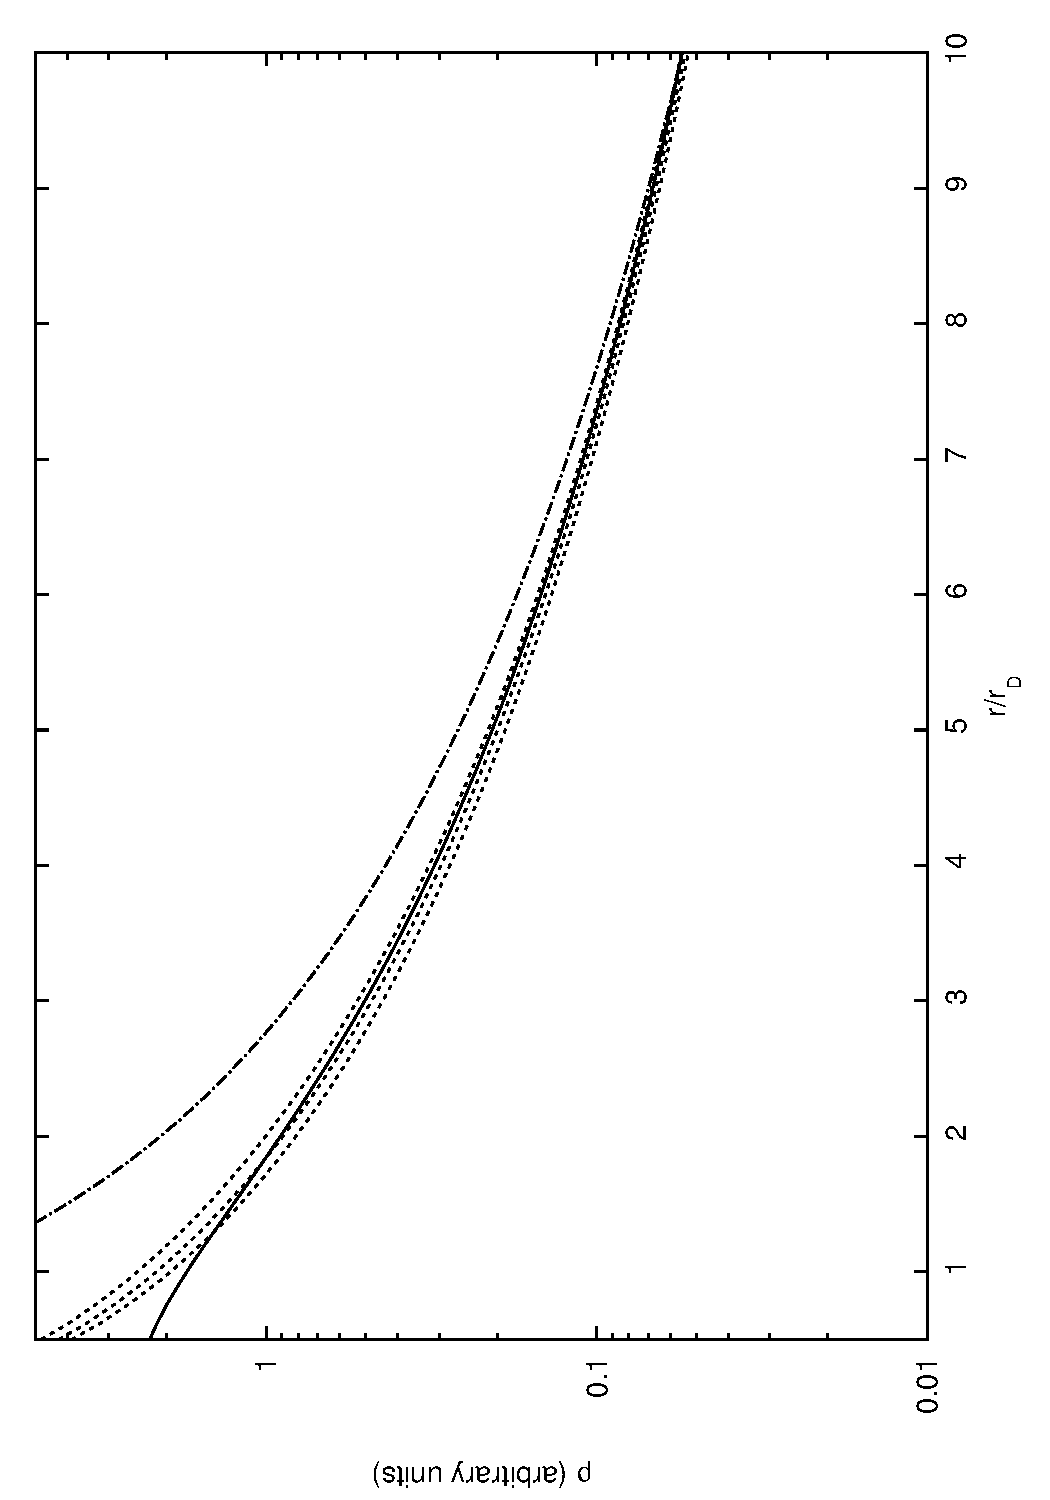
\includegraphics[scale=0.5, angle=270]{fig8}
  %      \rule{35em}{0.5pt}
    \caption{$\delta N _{\text{eff}}$[CMB] versus $\epsilon$ at fixed values of $m_{F_1}$ for (going from up to down) $m_{F_1}=0.1, 0.511, 0.7, 1, 10$ MeV.}
    \label{fig:Neffcmb}
\end{figure}
%
\begin{figure}[htpb]
   \vskip 0.2cm
    \centering
        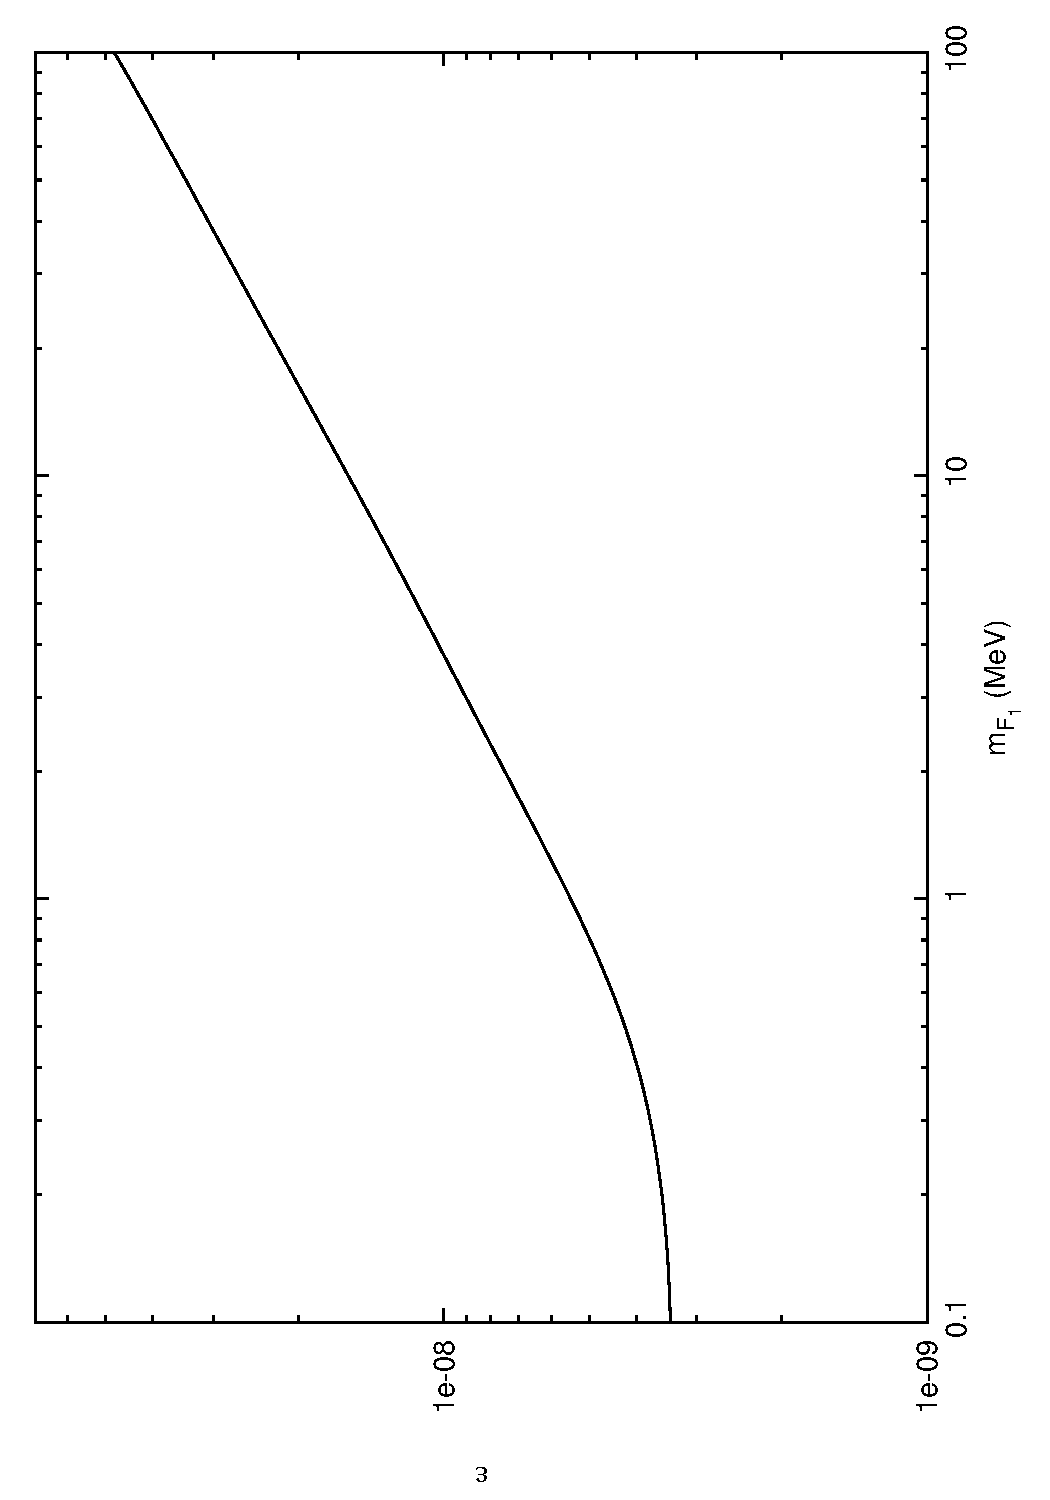
\includegraphics[scale=0.5, angle=270]{fig9}
%        \rule{35em}{0.5pt}
    \caption{Exclusion limits obtained from $\delta N _{\text{eff}}$[CMB] $<$ 0.84 in $\epsilon$-$m_{F_1}$ parameter space (excluded region is above line).}
    \label{fig:Exclusion cmb}
\end{figure}
%
\newpage
%
\subsection{Calculation of $\delta N _{\text{eff}}$[BBN]}

The addition of extra energy density during the early Universe also has an effect on BBN, the process during which light nuclei, and in particular helium, were synthesized (for a more detailed review see e.g. \cite{weinberg}). It is known that increasing the energy density by the addition of one neutrino species increases the helium fraction, $Y _p$, by approximately 0.013 \cite{bernstein}. It follows therefore that the change in the effective number of neutrino species associated with BBN is approximately given by:
%
\begin{eqnarray}
\delta N _{\text{eff}}[\text{BBN}] = \frac{Y _p (\epsilon) - Y _p (\epsilon = 0)}{0.013} \ .
\label{Neffbbn}
\end{eqnarray}
%
The first step towards the synthesis of helium is the synthesis of deuterium which, in turn, depends on the neutron abundance $X _n \equiv n _p/(n _n + n _p)$. We begin by considering the weak interaction processes which affect the neutron abundance:
%
\begin{eqnarray}
n + \nu _e \leftrightarrow p + e \ , \nonumber \\
n + \bar e \leftrightarrow p + \bar \nu _e \ , \nonumber \\
n \rightarrow p + e + \bar \nu _e \ .
\end{eqnarray}
%
At equilibrium (hence, at high temperatures) $X _n \simeq 1/(1 + e^{Q/T})$, where $Q \simeq 1.293$ MeV is the difference between the neutron and the proton mass.

The rates for the four processes which affect the neutron abundance (excluding neutron decay) can be found in e.g. \cite{weinberg}:
%
\begin{eqnarray}
\lambda _1 & \equiv & \lambda (n + \nu _e \rightarrow p + e) = A \mathlarger \int ^{\infty}_{0} dP_{\nu} \ E_e^2 P_{\nu}^2 \frac{1}{e^{\frac{E_{\nu}}{T_{\nu}}}+1} \frac{1}{e^{-\frac{E_e}{T_{\gamma}}}+1} \ ,
\\
\lambda _2 & \equiv & \lambda (n + \bar e \rightarrow p + \bar \nu _e) = A \mathlarger \int ^{\infty}_{0} dP_e \ E_{\nu}^2 P_e^2 \frac{1}{e^{\frac{E_e}{T_{\gamma}}}+1} \frac{1}{e^{-\frac{E_{\nu}}{T_{\nu}}}+1} \ ,
\\
\lambda _3 & \equiv & \lambda (p + e \rightarrow n + \nu _e) = A \mathlarger \int ^{\infty}_{\sqrt{Q^2-m_e^2}} dP_e \ E_{\nu}^2 P_e^2 \frac{1}{e^{\frac{E_e}{T_{\gamma}}}+1} \frac{1}{e^{-\frac{E_{\nu}}{T_{\nu}}}+1} \ ,
\\
\lambda _4 & \equiv & \lambda (p + \bar \nu _e \rightarrow n + \bar e) = A \mathlarger \int ^{\infty}_{Q+m_e} dP_{\nu} \ E_e^2 P_{\nu}^2 \frac{1}{e^{\frac{E_{\nu}}{T_{\nu}}}+1} \frac{1}{e^{-\frac{E_e}{T_{\gamma}}}+1} \ ,
\end{eqnarray}
%
where $E _e$[$E _{\nu}$], $P _e$[$P _{\nu}$] indicate the electron [neutrino] energy and momentum respectively. The extremals of the integrals are obtained from kinematical considerations. The factors within the integral account for Fermi-Dirac statistics and Pauli blocking. The values of the various constants are given by:
%
\begin{eqnarray}
A & = & \frac{G_F^2 (1+3g_A^2)\cos ^2\theta _c}{2\pi ^3} \ , \nonumber \\
G_F & = & 1.166 \times 10^{-5} \ {\rm GeV^{-2}} \ , \nonumber \\
g_A & = & 1.257 \ , \nonumber \\
\cos \theta _c & = & 0.97456 \ .
\end{eqnarray}
%
The evolution of $X _n$ is governed by the differential equation:
%
\begin{eqnarray}
\frac{dX _n}{dt} = -( \lambda _1 + \lambda _2 + \lambda _n)X _n + (\lambda _3 + \lambda _4)(1 - X _n) \ ,
\label{neutron}
\end{eqnarray}
%
where $\lambda _n ^{-1} = \tau _n \simeq 886.7 \ \rm s$ is the neutron lifetime. Eq.(\ref{neutron}) can be used to evolve the neutron fraction down to the so-called \textit{deuterium bottleneck} temperature $T _{\gamma} \simeq$ 0.07 MeV (of course, Eqs.(\ref{friedmannbis},\ref{sistema1}) need to be solved simultaneously to obtain the modified time-temperature relation). The helium fraction, $Y _p$, is twice the value of $X _n$ at this time, and $\delta N _{\text{eff}}$[BBN] can be evaluated by using Eq.(\ref{Neffbbn}).

There are hints that $\delta N _{\text{eff}}$[BBN] is also non-zero and positive. The data constrains $\delta N _{\text{eff}}[\text{BBN}] < 1$ at around 95\% confidence level \cite{izotov}. In Figure \ref{fig:Neffbbnmf1} $\delta N _{\text{eff}}$[BBN] is plotted against $\epsilon$ keeping $m _{F_1}$ fixed. The constraints following from this analysis are shown together with those obtained from $\delta N _{\text{eff}}$[CMB] in Figure \ref{fig:Comparison bbn cmb}. Evidently the limits set by $\delta N _{\text{eff}}$[CMB] are more stringent than those set by $\delta N _{\text{eff}}$[BBN]. Finally, we find an analytic approximation to CMB $\delta N _{\text{eff}}$ constraints on $\epsilon$ arising from early Universe cosmology:
%
\begin{eqnarray}
\epsilon \lesssim 3.5 \times 10 ^{-9} \left ( \frac{{\cal M}}{m _e} \right ) ^{\frac{1}{2}} \ .
\label{constraints}
\end{eqnarray}
%
The $\epsilon \sim {\cal M} ^{\frac{1}{2}}$ dependence can easily be understood by referring to Eqs.(\ref{masterformula},\ref{Neffcmb}).

\vskip 2 cm
%
\begin{figure}[htpb]
    \centering
        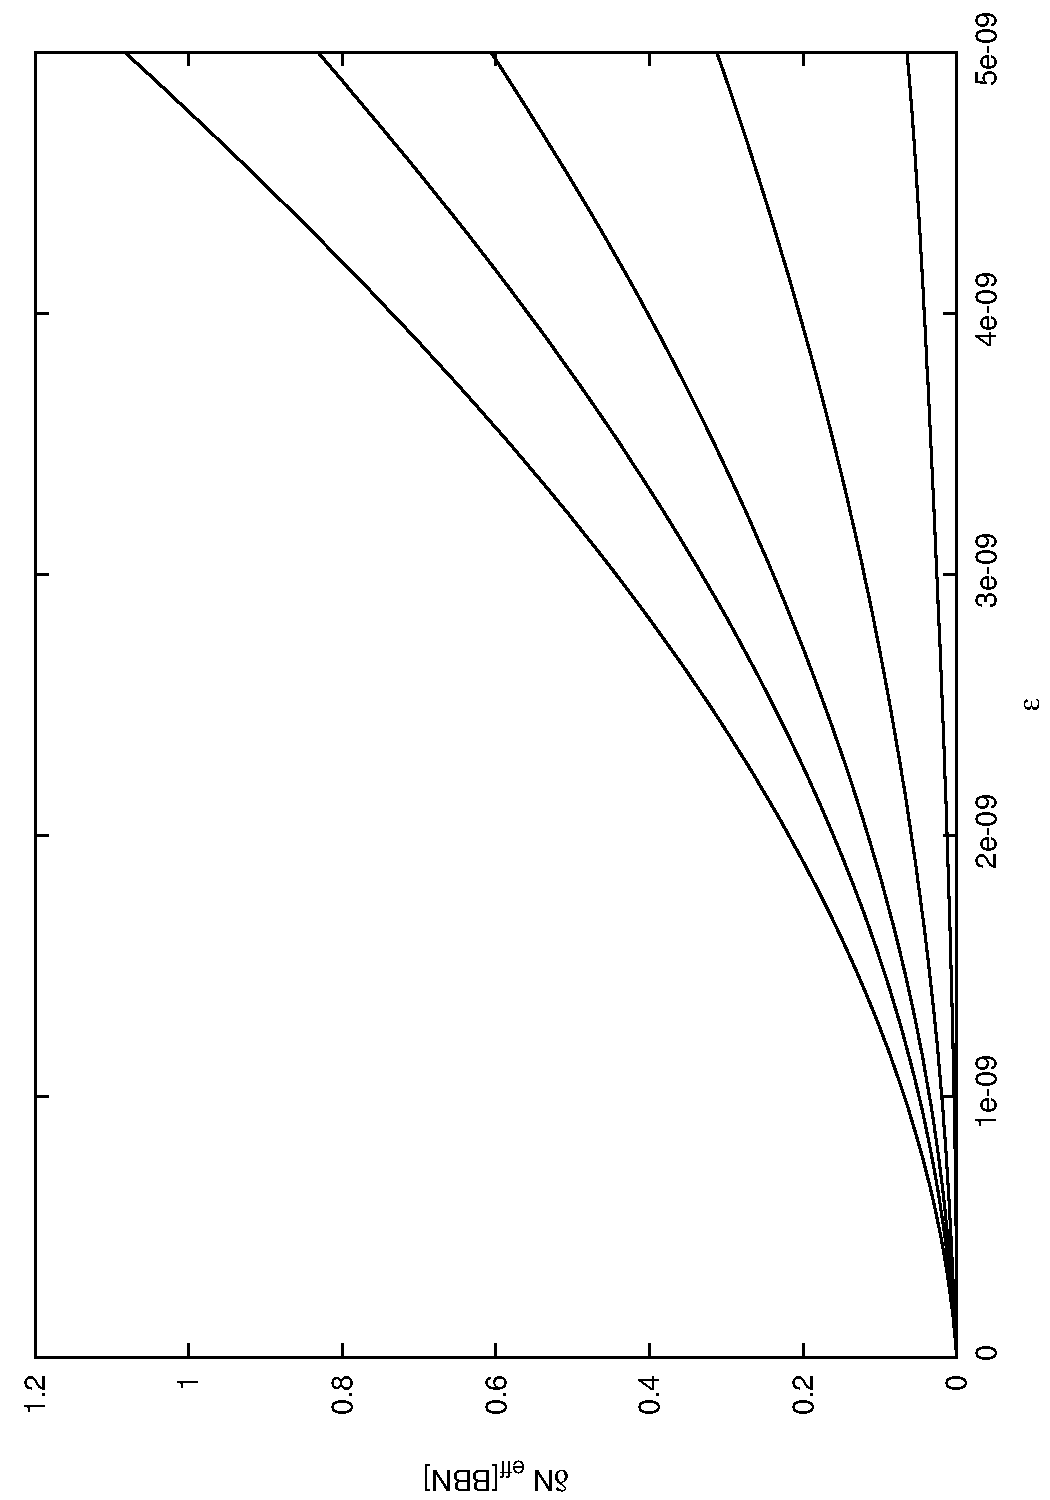
\includegraphics[scale=0.5, angle=270]{fig4bis}
%        \rule{35em}{0.5pt}
    \caption{$\delta N _{\text{eff}}$[BBN] versus $\epsilon$ at fixed values of $m_{F_1}$ for (going from up to down) $m _{F_1} = 0.1, 0.7, 1, 2, 10$ MeV.}
    \label{fig:Neffbbnmf1}
\end{figure}
%
\begin{figure}[htpb]
    \centering
        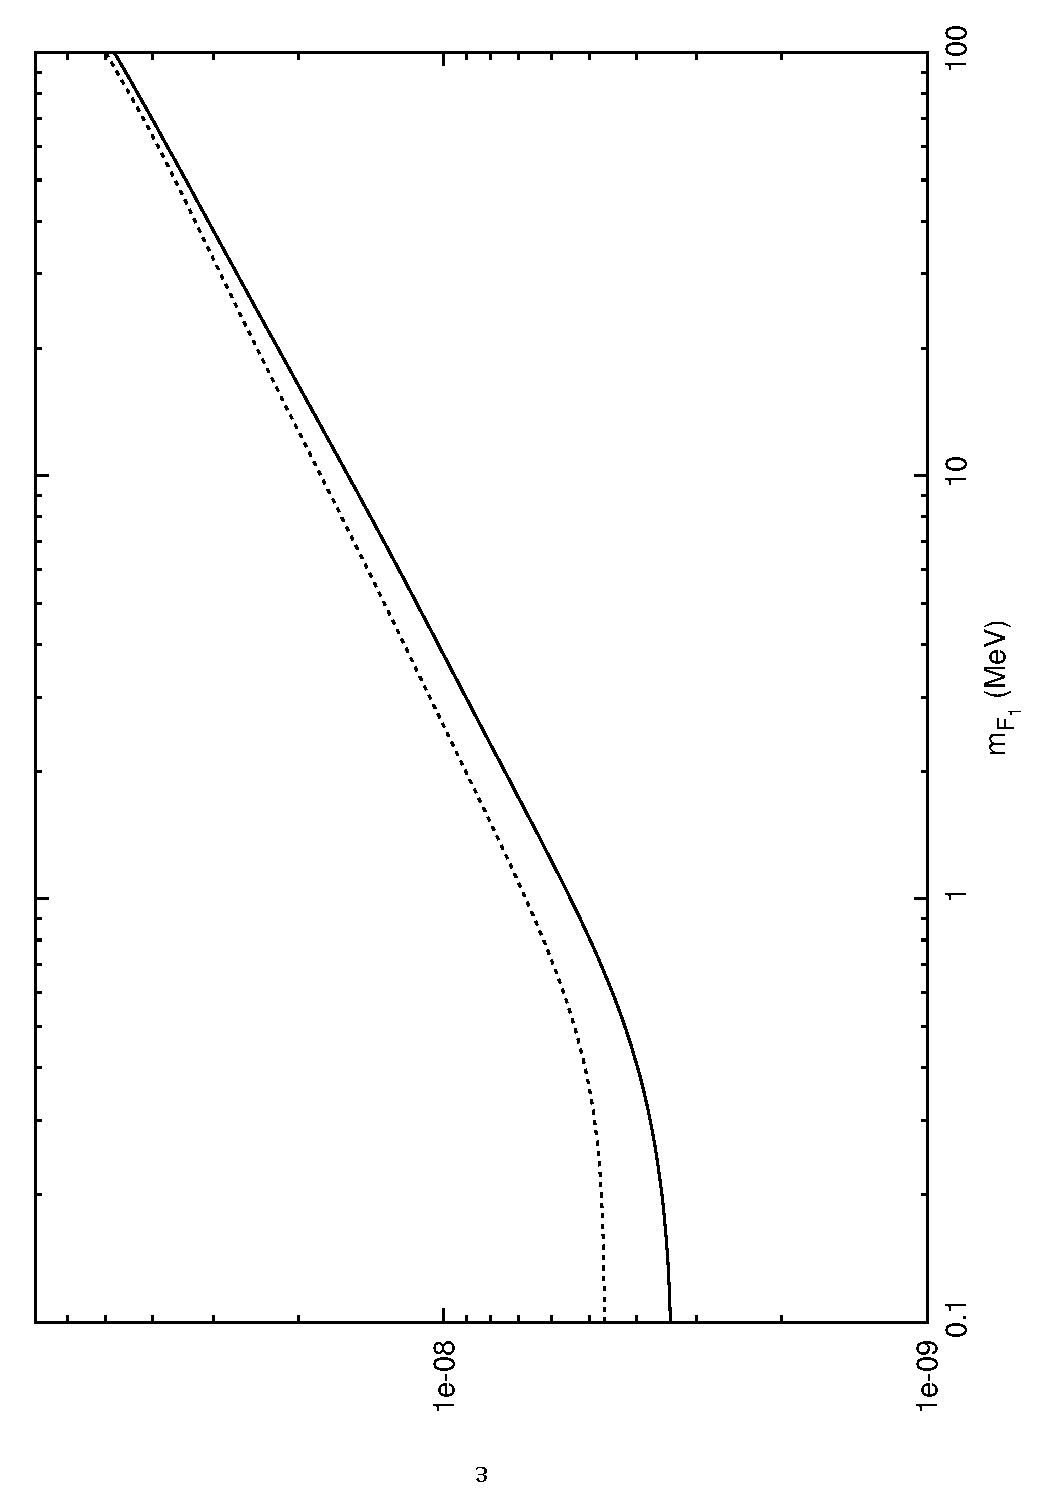
\includegraphics[scale=0.5, angle=270]{fig10}
%        \rule{35em}{0.5pt}
    \caption{Exclusion limits from $\delta N _{\text{eff}}$[CMB] $<$ 0.84 (solid line) and $\delta N _{\text{eff}}$[BBN] $<$ 1 (dashed line). Region above lines are excluded.}
    \label{fig:Comparison bbn cmb}
\end{figure}
%

\newpage

\section{Dark recombination}

\subsection{Saha equation for dark recombination}

Additional energy density, as parametrized by $\delta N _{\text{eff}}$[CMB], is not the only new physics affecting the CMB. Prior to recombination of $F _1$ and $F _2$ into neutral dark states, dark matter behaves like a tightly coupled fluid which undergoes dark acoustic oscillations. These oscillations suppress power on small scales (hence deviating from collisionless CDM), below some characteristic scale $L ^{\star}$, which is itself a function of the parameters in our model. Ultimately such a suppression of power on small scales may help in explaining the observed dearth of small galaxies in the neighborhood of the Milky Way. In the following, though, we simply derive approximate bounds by requiring that $T _{\text{dr}} \gtrsim T _{\text{eq}}$, where $T _{\text{dr}}$ is the temperature in the visible sector at the time of \textit{dark recombination}, and $T _{\text{eq}}$ is the temperature of matter-radiation equality. This requirement has been used in the literature (see for instance \cite{volkaspetraki}), and follows from studies in the MDM context \cite{berezhiani,implications,cia}. Roughly, $T _{\text{dr}} \gtrsim T _{\text{eq}}$ means that LSS is unaffected by dark acoustic oscillations on scales which are still growing linearly today.

In the present model, \textit{dark recombination} involves $|Z ^{'}|$ $F _1$ particles combining with one $F _2$ particle to form a $U(1) ^{'}$-neutral dark state, which will be called $D ^0$ (recall $Z ^{'}$ is the charge ratio of $F _2$ and $F _1$). We would like to know when (at what temperature or, equivalently, redshift) does dark recombination happen, that is, the moment in which the \textit{last} $F _1$ recombines with the state formed by $|Z ^{'}|$-1 $F _1$ particles and one $F _2$. Let us call this last state $D ^+$ (we take the convention where $F _1$ has charge -1 and $F _2$ has charge $|Z'|$). The relevant process to look at is:
%
\begin{eqnarray}
F _1 + D ^+ \leftrightarrow D ^0 + \gamma _{_D} \ .
\end{eqnarray}
%
The Saha equation for the process above is given in e.g. \cite{dodelson}:
%
\begin{eqnarray}
\frac{n _{D ^0}}{n _{D ^+} n _{F_1}} = \frac{{n _{D ^0}}^{(0)}}{{n_{D ^+}}^{(0)}{n _{F_1}}^{(0)}} \ ,
\label{Saha}
\end{eqnarray}
%
where the superscript $^{(0)}$ denotes the equilibrium value. Note that in writing Eq.(\ref{Saha}) it has been assumed $n _{\gamma _{_D}} = {n _{\gamma _{_D}}} ^{(0)}$. It is worth stressing that Eq.(\ref{Saha}) is an approximate equilibrium equation, namely, the equilibrium limit of the Boltzmann equations. It does not, therefore, follow the abundances through out-of-equilibrium processes, such as freeze-out (see for instance \cite{dodelson}). Eq.(\ref{Saha}), nonetheless, predicts the correct redshift of dark recombination, which is the quantity we wish to determine.

To proceed, it is useful to introduce the ionization fraction of $F _1$:
%
\begin{eqnarray}
\chi \equiv \frac{n _{F_1}}{n _{F_2}} = \frac{n _{F_1}}{n _{F_1} + n _{D ^0}} = \frac{n _{F_1}}{n _{D ^+} + n _{D ^0}} \ ,
\end{eqnarray}
%
where $n _{F_1}$ is the number density of free $F_1$ particles and $n _{F_2}$ is the total number density of $F_2$. The last equality follows from assuming $U(1) ^{'}$ neutrality. The left-hand side of Eq.(\ref{Saha}) is then $(1-\chi)/(n _{F_2}\chi ^2)$. The right-hand side of Eq.(\ref{Saha}) can also be expressed in a more useful form. For a species $A$ of mass $m _A$ and temperature $T _A$, the equilibrium number density in the limit $m _A \gg T _A$ can be written as (see e.g. \cite{dodelson}):
%
\begin{eqnarray}
n _A = g _A \left ( \frac{m _A T _A}{2\pi} \right ) ^{\frac{3}{2}} e ^{-\frac{m _A - \mu _A}{T _A}} \ ,
\end{eqnarray}
%
with $\mu _A$ being the chemical potential of the species and $g _A$ a degeneracy factor that usually takes into account multiple spin states. To good approximation $\mu _{\gamma _{_D}} = 0$ so, as long as equilibrium holds, the following is true:
%
\begin{eqnarray}
\mu _{F_1} + \mu _{D ^+} = \mu _{D ^0} \ .
\end{eqnarray}
%
The ionization energy of $D ^0$, $I ^{'}$, is defined to be:
%
\begin{eqnarray}
I ^{'} = m _{F_1} + m _{D ^+} - m _{D ^0} \ .
\end{eqnarray}
%
Eq.(\ref{Saha}) can be rearranged in a form which is more useful for following the evolution of the ionization fraction of $F _1$. To do so, we can employ the fact that $g _{F_1}g _{D ^+} = g _{D ^0}$ and work in the approximation $m _{D ^+} \simeq m _{D ^0}$. This approximation is valid as long as $m _{F_2} \gg m _{F_1}$ which is assumed. These considerations allow the right-hand side of Eq.(\ref{Saha}) to be rearranged to the form:
%
\begin{eqnarray}
\frac{{n _{D ^0}}^{(0)}}{{n_{D ^+}}^{(0)}{n _{F_1}}^{(0)}} = \left ( \frac{2\pi}{m _{F_1}T _{\gamma _{_D}}} \right ) ^{\frac{3}{2}} e ^{\frac{I ^{'}}{T _{\gamma _{_D}}}} \ .
\label{Saha1}
\end{eqnarray}
%
The end result is that the Saha equation [Eq.(\ref{Saha})] can be reduced to the more suitable form:
%
\begin{eqnarray}
\frac{1 - \chi}{\chi ^2} = n _{F_2}\left ( \frac{2\pi}{m _{F_1}T _{\gamma _{_D}}} \right ) ^{\frac{3}{2}} e ^{\frac{I ^{'}}{T _{\gamma _{_D}}}} \ .
\label{Saha2}
\end{eqnarray}
%
The $F _2$ number density simply scales as the baryon number density:
%
\begin{eqnarray}
n _{F_2} = \left ( \frac{\Omega _{\text{dm}}}{\Omega _{\text b}} \right ) \left ( \frac{m _p}{m _{F_2}} \right ) n _B = \left ( \frac{\Omega _{\text{dm}}}{\Omega _{\text b}} \right ) \left ( \frac{m _p}{m _{F_2}} \right ) \left ( \frac{n _B}{n _{\gamma}} \right ) \left ( \frac{n _{\gamma}}{n _{\gamma _{_D}}} \right ) n _{\gamma _{_D}} \ ,
\label{nf2scale}
\end{eqnarray}
%
where $m _p \simeq 0.94 \ {\rm GeV}$ is the proton mass and $\eta \equiv n _B/n _{\gamma}$ is the baryon-to-photon ratio. Using $\Omega _{\text{dm}}/\Omega _{\text b} \simeq 5.4$ \cite{plax}, $\eta \simeq 6 \times 10 ^{-10}$ \cite{pdg}, $n _{\gamma}/n _{\gamma _{_D}} = \left (T _{\gamma}/T _{\gamma _{_D}} \right ) ^3$ [with $T _{\gamma}/T _{\gamma _{_D}}$ evaluated using Eq.(\ref{masterformula})] and $n _{\gamma _{_D}} = \pi ^2T _{\gamma _{_D}} ^3/45$ allows us to rewrite Eq.(\ref{Saha2}) in the following form:
%
\begin{eqnarray}
\frac{1 - \chi}{\chi ^2} = A \left ( \frac{T _{\gamma _{_D}}}{I ^{'}} \right ) ^{\frac{3}{2}} e ^{\frac{I ^{'}}{T _{\gamma _{_D}}}} \ ,
\label{Saha23}
\end{eqnarray}
%
where:
%
\begin{eqnarray}
A \simeq 3.5 \times 10 ^{-7} \left ( \frac{10 ^{-9}}{\epsilon} \right ) ^{\frac{3}{2}} \left ( \frac{{\cal M}}{m _e} \right ) ^{\frac{3}{4}} \left ( \frac{\rm GeV}{m _{F_2}} \right ) \left ( \frac{I ^{'}}{m _{F_1}} \right ) ^{\frac{3}{2}} \ .
\end{eqnarray}
%
Using the variable $\xi \equiv I ^{'}/T _{\gamma _{_D}}$, Eq.(\ref{Saha23}) can be put to the form:
%
\begin{eqnarray}
\frac{1 - \chi}{\chi ^2} = A \xi ^{-\frac{3}{2}} e ^{\xi} \ .
\label{Saha3}
\end{eqnarray}
%
The Saha equation can be used to determine the redshift of dark recombination. To solve for the redshift (or, equivalently, temperature) of dark recombination, we take $\chi \approx 0.1$, so that Eq.(\ref{Saha3}) reduces to:
%
\begin{eqnarray}
\xi = \frac{3}{2} \ln \xi + \ln \left ( \frac{90}{A} \right ) \ .
\label{sahafinal}
\end{eqnarray}
%
In this form the Saha equation is easy to solve numerically. Once  the value of $\xi$ that solves the equation has been found, the temperature of the dark sector at dark recombination, $T _{\text{dr}} ^{'}$, is given by:
%
\begin{eqnarray}
T _{\text{dr}} ^{'} = \frac{I ^{'}}{\xi} \ .
\label{tdark}
\end{eqnarray}
%
The corresponding temperature of the visible sector at the time of dark recombination, $T _{\text{dr}}$, can be found by inverting Eq.(\ref{masterformula}):
%
\begin{eqnarray}
T _{\text{dr}} \simeq 3.2 \ T _{\text{dr}} ^{'} \left ( \frac{10 ^{-9}}{\epsilon} \right ) ^{\frac{1}{2}} \left ( \frac{{\cal M}}{m _e} \right ) ^{\frac{1}{4}} \ .
\label{darkord}
\end{eqnarray}
%
\subsection{Binding energy of the dark bound state}

To make progress, we need to determine $I ^{'}$ in terms of the parameters of our model. The bound system of $F _2$ with $N$ $F _1$ particles is completely analogous to that of nuclei with $N$ electrons. It follows that the binding energy of the dark state has the general form:
%
\begin{eqnarray}
I ^{'} = {Z _{\text{eff}}'} ^2 \frac{\alpha '^{2}}{2} \mu _R \ ,
\label{ip}
\end{eqnarray} 
%
where $\mu _R$ is the reduced mass of the $F_1$-$D ^+$ system, given by $\mu _R = m _{F_1}m _{D ^+}/(m _{F_1} + m _{D ^+})$. In the limit where $m _{F_2} \gg m _{F_1}$ one has that $I ^{'} \simeq Z _{\text{eff}} ^{'2} \ {\alpha '} ^2 m _{F_1}/2$.

Naturally exact analytic expressions for $Z _{\text{eff}} ^{'}$ are in general unknown, but it is still possible to make a rough approximation for $Z ^{'} _{\text{eff}}$ and hence determine $I ^{'}$. The charge $Z _{\text{eff}} ^{'}$ depends only on the chemistry (or equivalently on quantum mechanics) of the bound state we are analyzing. In particular, it depends on shielding effects due to the $|Z ^{'}|$-$1$ $F _1$ particles partially shielding the charge of the $F _2$ particle from the last $F _1$ which is about to combine. The problem of determining $Z _{\text{eff}} ^{'}$ is therefore identical to that of determining the shielding of an ordinary nucleus of atomic number $Z = |Z ^{'}|$ due to $Z$-$1$ electrons. It essentially only depends on the way the fermions arrange themselves in orbitals, which in turn is determined solely by quantum mechanics.

Under these assumptions the binding energy $I ^{'}$ of the dark bound state can be derived simply by scaling the binding energy $I$ of the corresponding ordinary element with atomic number $Z = |Z ^{'}|$ via:
%
\begin{eqnarray}
I ^{'} = \left ( \frac{\alpha ^{'}}{\alpha} \right ) ^2 \left ( \frac{m _{F_1}}{m _e} \right ) I \ .
\label{scaling}
\end{eqnarray}
%
A plot of the binding energies of the elements of the periodic table as a function of the atomic number $Z$ is shown in Figure \ref{fig:Ionization}. One notes from Figure \ref{fig:Ionization} that, apart from isolated cases such as He, the binding energies of the various elements reside in a fairly narrow range centered at about $10$ eV, within a factor of approximately 2. For $Z \gtrsim 10$, the dependence of $I$ on $Z$ is even weaker. This means that $Z _{\text{eff}} ^{'} \approx 1$ in Eq.(\ref{ip}) and $I ^{'} \approx {\alpha '} ^2m _{F_1}/2$.

\vskip 1 cm

%
\begin{figure}[htpb]
    \centering
        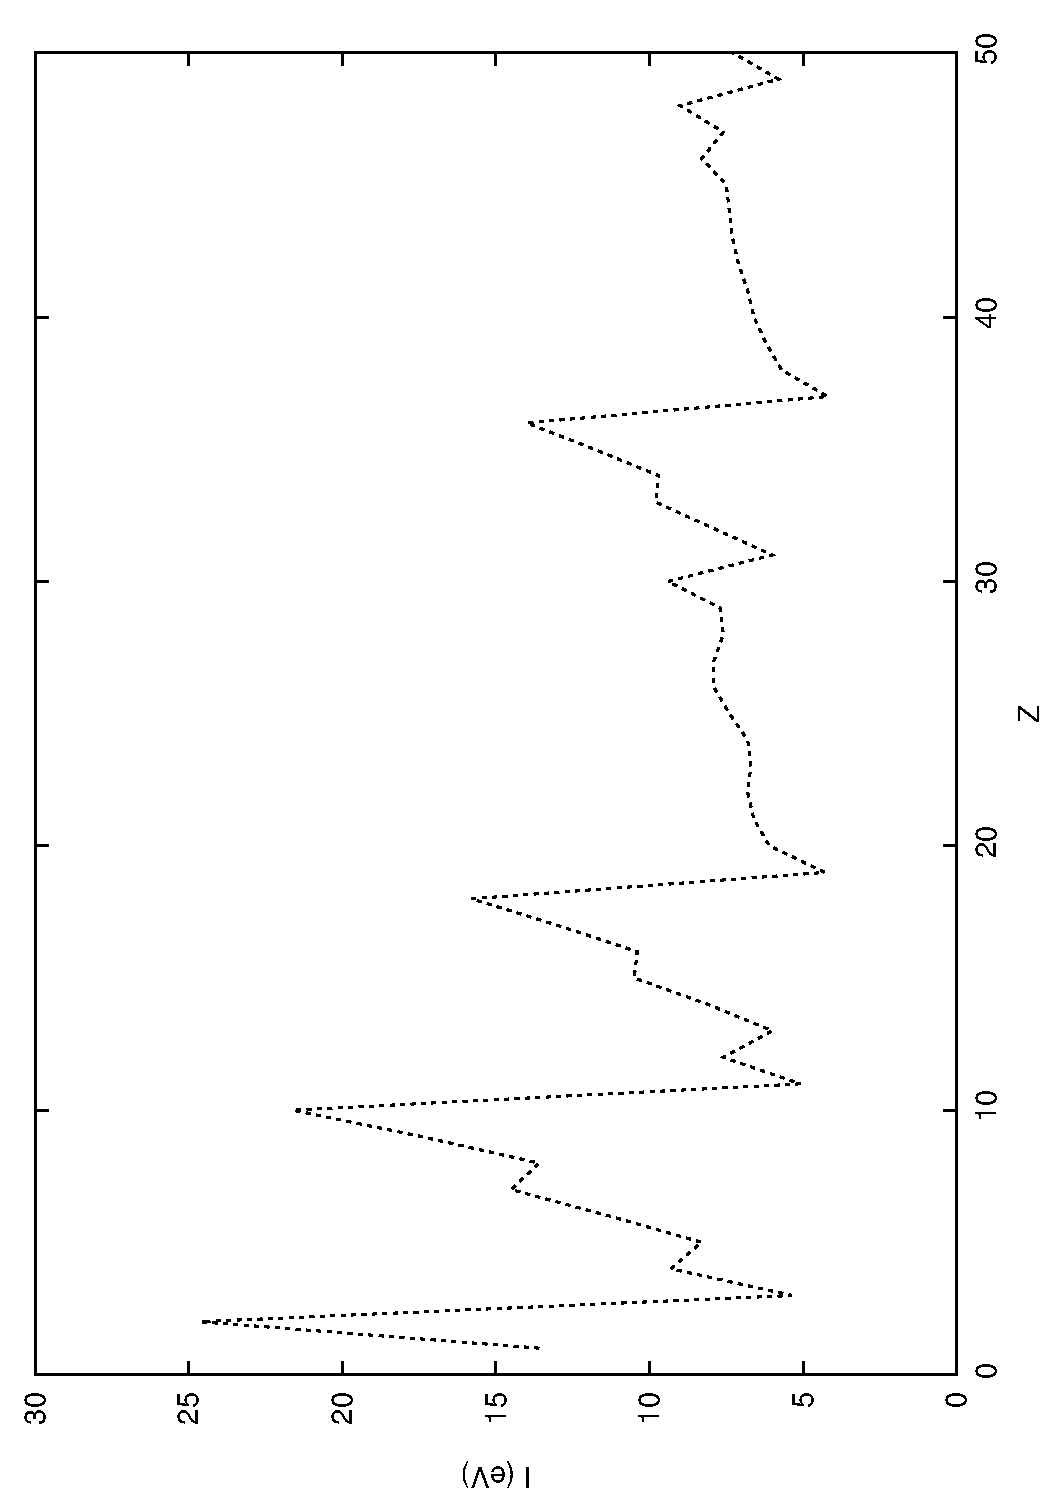
\includegraphics[scale=0.45, angle=270]{ionization}
%        \rule{35em}{0.5pt}
    \caption{Ionization energy as a function of atomic number for ordinary elements.}
    \label{fig:Ionization}
\end{figure}
%
\newpage

\subsection{Exclusion limits}

Recall the validity of our model requires $T _{\text{dr}} \gtrsim T _{\text{eq}}$, where $T _{\text{eq}}$ is the temperature of the visible sector at matter-radiation equality. This condition is required for successful LSS formation (e.g. \cite{volkaspetraki}). The redshift of matter-radiation equality is $z _{\text{eq}} = 3200 \pm 130$ \cite{pdg}, which leads to a lower limit on the matter-radiation equality temperature of about $T _{\text{eq}} = 0.72$ eV.

We can now scan the parameter space of this model and set constraints on its parameters. In principle the model presents five parameters : $m _{F_1}$, $m _{F_2}$, $\alpha ^{'}$, $\epsilon$ and $Z ^{'}$. A numerical analysis of the solution, $T _{\text{dr}} \gtrsim T _{\text{eq}}$, manifests a weak dependence on $m _{F_2}$. This can be understood by noting that an iterative solution of Eq.(\ref{sahafinal}) displays a log-like dependence on the value of the constant $A$, which is the only place where $m _{F_2}$ comes into play. The dependence on $Z ^{'}$ is also relatively minor, since as previously noted it only affects the binding energy in a modest way.

To summarize, the physics of dark recombination, to a rough approximation, depends on just 3 parameters: $m _{F_1}$, $\alpha ^{'}$ and $\epsilon$ (being relatively insensitive to $Z'$ and $m _{F_2}$). We now derive constraints on these 3 parameters.

\begin{figure}[htpb]
    \centering
        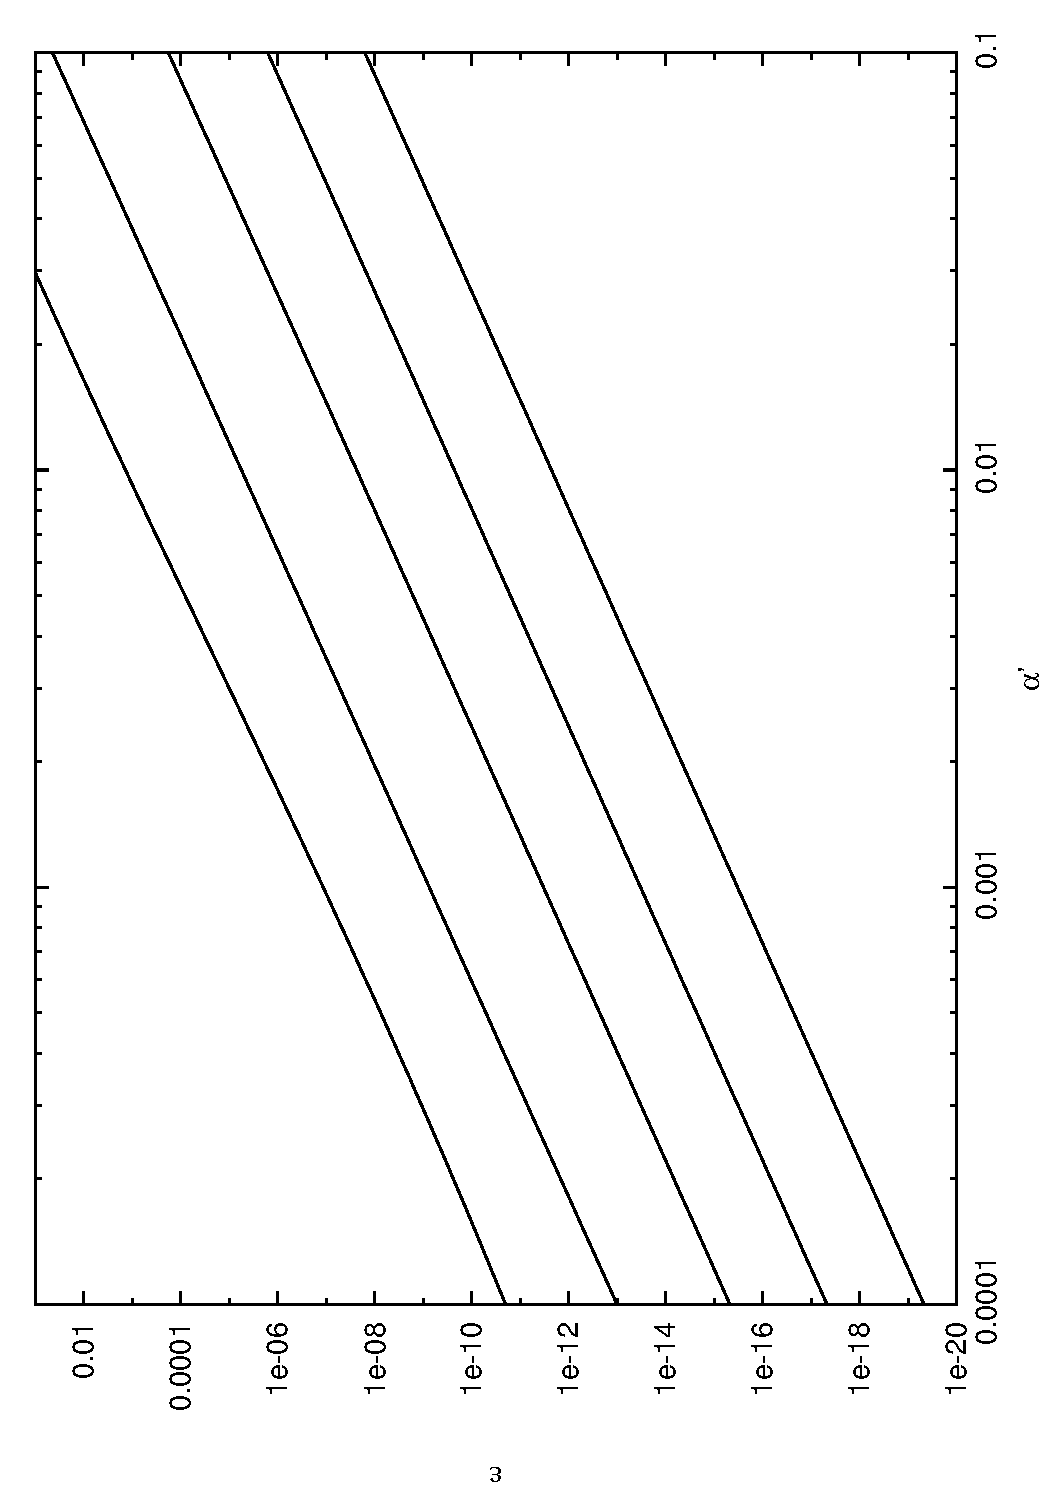
\includegraphics[scale=0.5, angle=270]{fig11}
%        \rule{35em}{0.5pt}
    \caption{Exclusion limits from the constraint on the temperature of dark recombination (discussed in text). The limits are for fixed values of $m _{F_1}$ for (going from upper to lower line) $m _{F_1} = 100, 10, 1, 0.1, 0.01$ MeV (excluded region is above the line).}
    \label{fig:Exclusion dark recombination mf1}
\vskip 1cm
\end{figure}


As already discussed, we derive exclusion limits by requiring $T _{\text{dr}} \gtrsim T _{\text{eq}}$, and using Eqs.(\ref{sahafinal},\ref{tdark},\ref{darkord},\ref{scaling}) [we take $I = 10 \ {\rm eV}$ in Eq.(\ref{scaling})]. In Figure \ref{fig:Exclusion dark recombination mf1} we give the results for a fixed $m _{F_1}$ and varying $\alpha ^{'}$. The dependence on $\alpha ^{'}$, $m _{F_1}$ shown in Figure \ref{fig:Exclusion dark recombination mf1} can be easily understood by analytical considerations. Recall, to constrain the model we look for the value of parameters for which $T _{\text{dr}} \gtrsim T _{\text{eq}} \simeq 0.72$ eV. From Eqs.(\ref{tdark},\ref{scaling}) we have that $T ^{'} \propto I ^{'} \propto {\alpha '} ^2 m _{F_1}$, while Eq.({\ref{masterformula}) implies $T _{\text{dr}} = T _{\text{dr}} ^{'}T _{\text{dr}}/T _{\text{dr}} ^{'} \propto {\alpha '} ^2m _{F_1}{\cal M} ^{\frac{1}{4}}/\sqrt{\epsilon}$. It follows therefore that the upper limit on $\epsilon$ scales as ${\alpha '} ^4 m _{F_1} ^2\sqrt{\cal M}$. In fact, the numerical results shown in Figure {\ref{fig:Exclusion dark recombination mf1} give the upper bound on $\epsilon$, coming from dark recombination:
%
\begin{eqnarray}
\epsilon \lesssim 10 ^{-8} \left ( \frac{\alpha '}{\alpha} \right ) ^4 \left ( \frac{m _{F_1}}{\rm MeV} \right ) ^2 \left ( \frac{{\cal M}}{m _e} \right ) ^{\frac{1}{2}} \ .
\label{boundse}
\end{eqnarray}
% 
The above upper bound also includes a factor of $\sim$ 2 uncertainty on $\epsilon$ arising from the uncertainty on $I$ [$I = (10 \pm 5) \ {\rm eV}$].

\section{Galactic structure}

\subsection{Dynamical halo model and halo scaling relations}

The physical picture of spiral galaxies is that of a flat disk of baryonic matter surrounded by a dark matter halo. In our model, the dark matter halo is formed by a plasma of $F _1$ and $F _2$ particles, where energy is lost to dissipative interactions, such as thermal dark bremsstrahlung. To account for the observed halo structure, a heat source that can replace this energy lost has to exist. In the MDM context, it has been argued that ordinary supernovae can supply this energy \cite{spheroidal,depth4,review}. The mechanism involves kinetic mixing induced processes ($e\overline{e} \rightarrow e'\overline{e}'$, $\gamma \rightarrow e'\overline{e}'$,...) in the supernovae core, which can convert $\sim 1/2$ of the core collapse energy into $\gamma ^{'}$, $e'$, $\overline{e}'$ for $\epsilon \sim 10 ^{-9}$ \cite{raf,updated} (see also \cite{silagadze}). Ultimately this energy is reprocessed into mirror photons in the region around the supernovae. Essentially the same mechanism can take place in our generic two-component dissipative dark matter model provided that $m _{F_1} \lesssim {\rm few} \times T _{\text{SN}} \approx 100 \ {\rm MeV}$.

The physical properties of the dark matter halo are then governed by the Euler equations of fluid dynamics, which take the form:
%
\begin{gather}
\frac{\partial \rho}{\partial t} + \nabla \cdot (\rho \mathbf{v}) = 0 \nonumber \ , \\
\frac{\partial \mathbf{v}}{\partial t} + (\mathbf{v} \cdot \nabla)\mathbf{v} = -\left ( \nabla \phi + \frac{\nabla P}{\rho} \right) \nonumber \ , \\
\frac{\partial}{\partial t} \left [\rho \left ( \frac{\mathbf{v}^2}{2} + {\cal E} \right ) \right ] + \nabla \cdot \left [\rho \left ( \frac{\mathbf{v}^2}{2} + \frac{P}{\rho} + {\cal E} \right ) \mathbf{v} \right ] - \rho \mathbf{v} \cdot \nabla \phi = \frac{d\Gamma _{\text{heat}}}{dV} - \frac{d\Gamma _{\text{cool}}}{dV} \ .
\label{euler}
\end{gather}
%
Here $P$, $\rho$ and $\mathbf{v}$ denote the pressure, mass density and velocity of the fluid. ${\cal E}$ is the internal energy per unit mass of the fluid, so that $\rho \left (\mathbf{v}^2/2 + {\cal E} \right )$ is the energy per unit volume. Finally, $\Gamma _{\text{heat}}$ and $\Gamma _{\text{cool}}$ are the heating and cooling rates. Significant simplifications occur if the system evolves to a static configuration. In this limit, all time derivatives in Eqs.(\ref{euler}) vanish, and if one also assumes spherical symmetry, then Eqs.(\ref{euler}) reduce to just two equations:
%
\begin{eqnarray}
\frac{d\Gamma _{\text{heat}}(r)}{dV} = \frac{d\Gamma _{\text{cool}}(r)}{dV} \ ,
\label{balance}
\end{eqnarray}
%
and
%
\begin{eqnarray}
\frac{dP(r)}{dr} = -\rho (r)g(r) \ .
\label{hydrostatic}
\end{eqnarray}
%
Here $g(r)=\nabla \phi$ is local gravitational acceleration.

The quantities $g(r)$, $P(r)$ can be related to the density $\rho (r)$ via:
%
\begin{eqnarray}
g(r) &=& \frac{v _{\text{rot}} ^2}{r} = \frac{G}{r ^2} \int _0 ^r dr' \ 4\pi {r'} ^2 \rho _T (r') \ , \nonumber \\
P(r) &=& \frac{\rho(r)T(r)}{\overline{m}} \ ,
\label{grhop}
\end{eqnarray}
%
where $\overline{m} = (n _{F_1}m _{F_1} + n _{F_2}m _{F_2})/(n _{F_1} + n _{F_2})$ is the mean mass of the particles forming the dark plasma and we have assumed local thermal equilibrium in order to relate $P$ to $T$. Here $\rho _T (r)$ is the total mass density which, in addition to the dark plasma component, $\rho (r)$, includes baryonic components (stars and gas) and possibly compact dark ``stars".

A few comments on Eqs.(\ref{balance},\ref{hydrostatic}) are in order. Eq.(\ref{balance}) represents energy balance at every point in the halo, while Eq.(\ref{hydrostatic}) is the hydrostatic equilibrium condition. Both conditions are required for a static configuration. Whether or not the system is able to evolve to such a static configuration is not certain, but seems possible. Assuming that the system, at an early time prior to the onset of ordinary star formation ($t \lesssim {\rm few} \ {\rm Gyr}$), was in a more compact configuration, then the subsequent star formation activity would expand and heat the halo (that is, $\Gamma _{\text{heat}} - \Gamma _{\text{cool}} > 0$ initially), which in turn would modify $\Gamma _{\text{heat}}-\Gamma _{\text{cool}}$ via various feedback processes. The idea is that these feedback processes can reduce $\Gamma _{\text{heat}} - \Gamma _{\text{cool}}$ as the halo expands until $\Gamma _{\text{heat}} - \Gamma _{\text{cool}} = 0$ is reached. For example, as the halo expands, the ordinary supernovae rate reduces in response to the weakening gravity, as expressed by the Schmidt-Kennicutt empirical law, which relates star formation rate to the gas density in spiral galaxies \cite{schmidt}:
%
\begin{eqnarray}
\dot{\Sigma} _{\star} \propto n _{\text{gas}} ^N \ , \ N \sim 1\text{-}2 \ .
\end{eqnarray}
%
This mechanism and others can potentially lead to a net reduction in $\Gamma _{\text{heat}} - \Gamma _{\text{cool}}$ as the halo expands, until eventually the static limit is reached where $\Gamma_{\text{heat}} = \Gamma_{\text{cool}}$.

In order to gain insight, we initially solve Eq.(\ref{hydrostatic}) assuming an isothermal halo, i.e. $dT/dr = 0$, and approximating $\rho _T (r) = \rho (r)$. Both of these approximations can be roughly valid in the outer regions of the galaxy. Combining Eqs.(\ref{hydrostatic},\ref{grhop}) and taking into account the isothermal approximation, the hydrostatic equilibrium equation can be expressed as:
%
\begin{eqnarray}
\frac{d\rho}{dr} = -\frac{\overline{m}\rho (r) G}{T r ^2}\int _0 ^r dr' \ 4\pi {r'} ^2 \rho (r') \ .
\label{hydrostatic1}
\end{eqnarray}
%
Eq.(\ref{hydrostatic1}) can be solved by a polynomial of the form $\rho = \lambda/r ^p$. Substitution into Eq.(\ref{hydrostatic1}) yields $p = 2$ and $\lambda = T/2\pi G\overline{m}$, that is:
%
\begin{eqnarray}
\rho (r) &=& \frac{T}{2\pi G\overline{m}r ^2} \ .
\label{ntrho}
\end{eqnarray}
%
Combining Eqs.(\ref{grhop},\ref{ntrho}) gives us the rotational velocity profile, which we can relate to the temperature of the halo:
%
\begin{eqnarray}
v _{\text{rot}} ^2 = \frac{G}{r}\int _0 ^r dr' \ 4\pi {r'} ^2\frac{T}{2\pi G\overline{m}{r'} ^2} = \frac{2T}{\overline{m}} \implies T = \frac{1}{2}\overline{m}v _{\text{rot}} ^2 \equiv \frac{1}{2}\overline{m}v _{\infty} ^2 \ .
\label{vrot}
\end{eqnarray}
%
The rotational velocity is found to be independent from the distance to the center of the galaxy, consistent with the observed asymptotically flat rotational curves of spiral galaxies, with asymptotic velocity $v _{\infty}$.

\subsubsection{Toy model}

Is the assumption of an isothermal halo justified? Let us consider a toy model, where we consider all supernovae as acting as a point source at the galactic centre ($r = 0$) producing a total dark photon luminosity $L _{\text{SN}}$. Clearly this model is unphysical, and will have to be refined later. To apply Eq.(\ref{balance}) to the system, we have to match the energies absorbed and dissipated within a volume element $dV$.

Supernovae are presumed to be a source of dark photons, resulting from kinetic mixing induced processes (e.g. $\gamma \rightarrow F_1\overline{F}_1$, $e\overline{e} \rightarrow F_1\overline{F}_1$) occurring in the supernovae cores. The resulting interactions in the region around the supernovae convert this energy into dark photons of uncertain spectrum. These dark photons can eventually escape and ultimately transport and inject the energy into the halo. Two possible mechanisms can be envised: dark photoionization and dark Thomson scattering. We show in Appendix B that dark Thomson scattering is an unimportant heating mechanism for the parameter space we are focusing on ($m _{F_1} \gtrsim 0.1 \ \rm MeV$).

Assuming, then, that the heating of the halo takes place via a dark photoionization process with cross-section $\sigma _{_{DP}}$, the energy per unit time being absorbed in a given volume element, $dV$, is given by:\footnote{In principle one has to integrate over the frequency spectrum of dark photons, as in \cite{depth4}, but this detail is not essential for the current discussion.}
%
\begin{eqnarray}
d\Gamma _{\text{heat}} = \frac{L _{\text{SN}}e ^{-\tau}}{4\pi r ^2}\sigma _{_{DP}}n _{F_2} dV \ ,
\label{ein}
\end{eqnarray}
%
where $\tau$ is the optical depth. We have assumed that the two K-shell atomic $F_1$ states are occupied, which means that the plasma cannot be completely ionized. We shall here assume that the remaining $(|Z'|-2)$ $F_1$ states are free, and will comment more on these consistency conditions in Section 5.2.2. Evidently, the validity of our model then requires $|Z'| \geq 3$.

Energy is lost via dark bremsstrahlung of $F _1$ off $F _2$. The energy dissipated per unit time within a volume element $dV$ is given by:
%
\begin{eqnarray}
d\Gamma _{\text{cool}} = \Lambda (T) n _{F_1}n _{F_2} dV \ ,
\label{eout}
\end{eqnarray}
%
where $\Lambda(T)$ is the cooling function for dark bremsstrahlung (defined more precisely in Section 5.2) and $n _{F_1}$ (henceforth) denotes the free $F_1$ particles number density. There are other sources of dissipation\footnote{One could also consider inverse Compton scattering, $F_1 \gamma _{_D} \rightarrow F_1 \gamma _{_D}$, where $\gamma _{_D}$ is a dark microwave background photon. For the range of parameter space and physical conditions we are examining, we find that inverse Compton scattering can be neglected except possibly at an early epoch, $z \gtrsim 3$.}, such as line emission and recombination, which could be included by modifying $\Lambda$ (see e.g. \cite{radiative}). Although they might be important, for the purposes of this discussion they will be neglected.\footnote{A more comprehensive discussion of cooling would have to take into account the cooling efficiency. In general not all bremsstrahlung dark photons will have mean free path sufficiently long as to escape the halo. Whether or not they can escape (and hence cool) the halo depends on their location of production and their wavelength. These effects could be incorporated by means of a cooling efficiency function which depends on these variables. However, such a discussion is beyond the scope of our paper and will be left for future work.} Matching of heating and cooling corresponds to equating the right-hand sides of Eqs.(\ref{ein},\ref{eout}), which yields:
%
\begin{eqnarray}
n _{F_1} = \frac{L _{\text{SN}}e ^{-\tau}}{\Lambda (T)4\pi r ^2}\sigma _{_{DP}} \ .
\label{match}
\end{eqnarray}
%
If, in addition, we make the assumption that the halo is optically thin ($\tau \ll 1$), we recover $n _{F_1} \propto 1/r ^2$. This also means that $\rho \propto 1/r ^2$.

The end result is that the assumption of an isothermal halo provides a solution to both energy balance [Eq.(\ref{balance})] and the hydrostatic equilibrium condition [Eq.(\ref{hydrostatic})]. This suggests that an isothermal halo can be a reasonable approximation at large distances from the galactic centre, where the supernova heat source can be modelled as a point source and where, in addition, $\rho _T (r) \simeq \rho (r)$.

\subsubsection{A refined model: solution to the core-cusp problem}

The toy model described above is unphysical at $r = 0$. To refine it, we smear the supernova energy source over a finite volume, on a distance scale $r_D$. Since we are dealing with ordinary supernovae, it is reasonable to assume they are distributed similarly to the mass of the galactic disk. One therefore expects the $\rho \propto 1/r ^2$ solution to hold only for $r \gg r _D$. The mass distribution of the galactic disk can be approximated by a profile known as Freeman disk, with surface density \cite{freeman}:
%
\begin{eqnarray}
\Sigma (\widetilde{r}) = \frac{m _D}{2\pi r_D ^2}e ^{-\frac{\widetilde{r}}{r_D}} \ ,
\end{eqnarray}
%
with $r_D$ being the disk scale length and $m _D$ its total mass. We can now follow the same steps as in \cite{review}. Using cylindrical coordinates ($\widetilde{r},\widetilde{\theta},\widetilde{z}$) and setting the disk at $\widetilde{z} = 0$, the flux at a point $P = (r _1,0,z _1)$ within an optically thin halo is given by:
%
\begin{eqnarray}
f(r,\cos \phi ) = \frac{L _{\text{SN}}}{4\pi m _D} \int d\widetilde{\theta} \int d\widetilde{r} \ \widetilde{r} \frac{\Sigma (\widetilde{r})}{{\widetilde{r}} ^2 - 2\widetilde{r}r _1 \cos \widetilde{\theta} + r _1 ^2 + z _1 ^2}
\end{eqnarray}
%
where $r = \sqrt{r _1 ^2 + z _1 ^2}$ and $\cos \phi \equiv r _1/r$. It is not hard to show that:
%
\begin{eqnarray}
f(r,\cos \phi) \propto \begin{cases}
                  \log r, & r \lesssim r_D \ , \\
                  \frac{1}{r ^2}, & r \gg r_D \ .
                  \end{cases}
\label{frc}
\end{eqnarray}
%
The energy lost per unit time due to thermal dark bremsstrahlung is once again given by Eq.(\ref{eout}), while the energy absorbed per unit time within a volume element $dV$ now takes the form:
%
\begin{eqnarray}
d\Gamma _{\text{heat}} = f(r,\cos \phi)\sigma _{_{DP}}n _{F _2}dV \ .
\label{ein1}
\end{eqnarray}
%

Again equating d$\Gamma _{\text{heat}}$=d$\Gamma _{\text{cool}}$, using Eqs.(\ref{eout},\ref{ein1}), implies $n _{F_1} = f(r,\cos \phi)\sigma _{_{DP}}/\Lambda (T)$. That is, $\rho \propto f(r,\cos \phi )$. The considerations given about the behavior of $f(r,\cos \phi)$ [Eq.(\ref{frc})] then suggest that $\rho (r)$ can be approximated by a quasi-isothermal dark matter profile:
%
\begin{eqnarray}
\rho (r) \simeq \frac{\rho _0r _0 ^2}{r ^2 + r _0 ^2} \ ,
\label{core}
\end{eqnarray}
%
where $r _0 \sim r_D$, since the latter is the only length scale present in the problem. In Figure \ref{fig:Comparison core f} we compare the radial dependence of the solution $\rho \propto f(r,\cos \phi)$ with the quasi-isothermal profile given by Eq.(\ref{core}), finding good agreement up to $r \simeq r _D$, when the contribution of baryons dominates over the dark matter and hence cannot be neglected.

\begin{figure}[htpb]
    \vskip 1cm
    \centering
        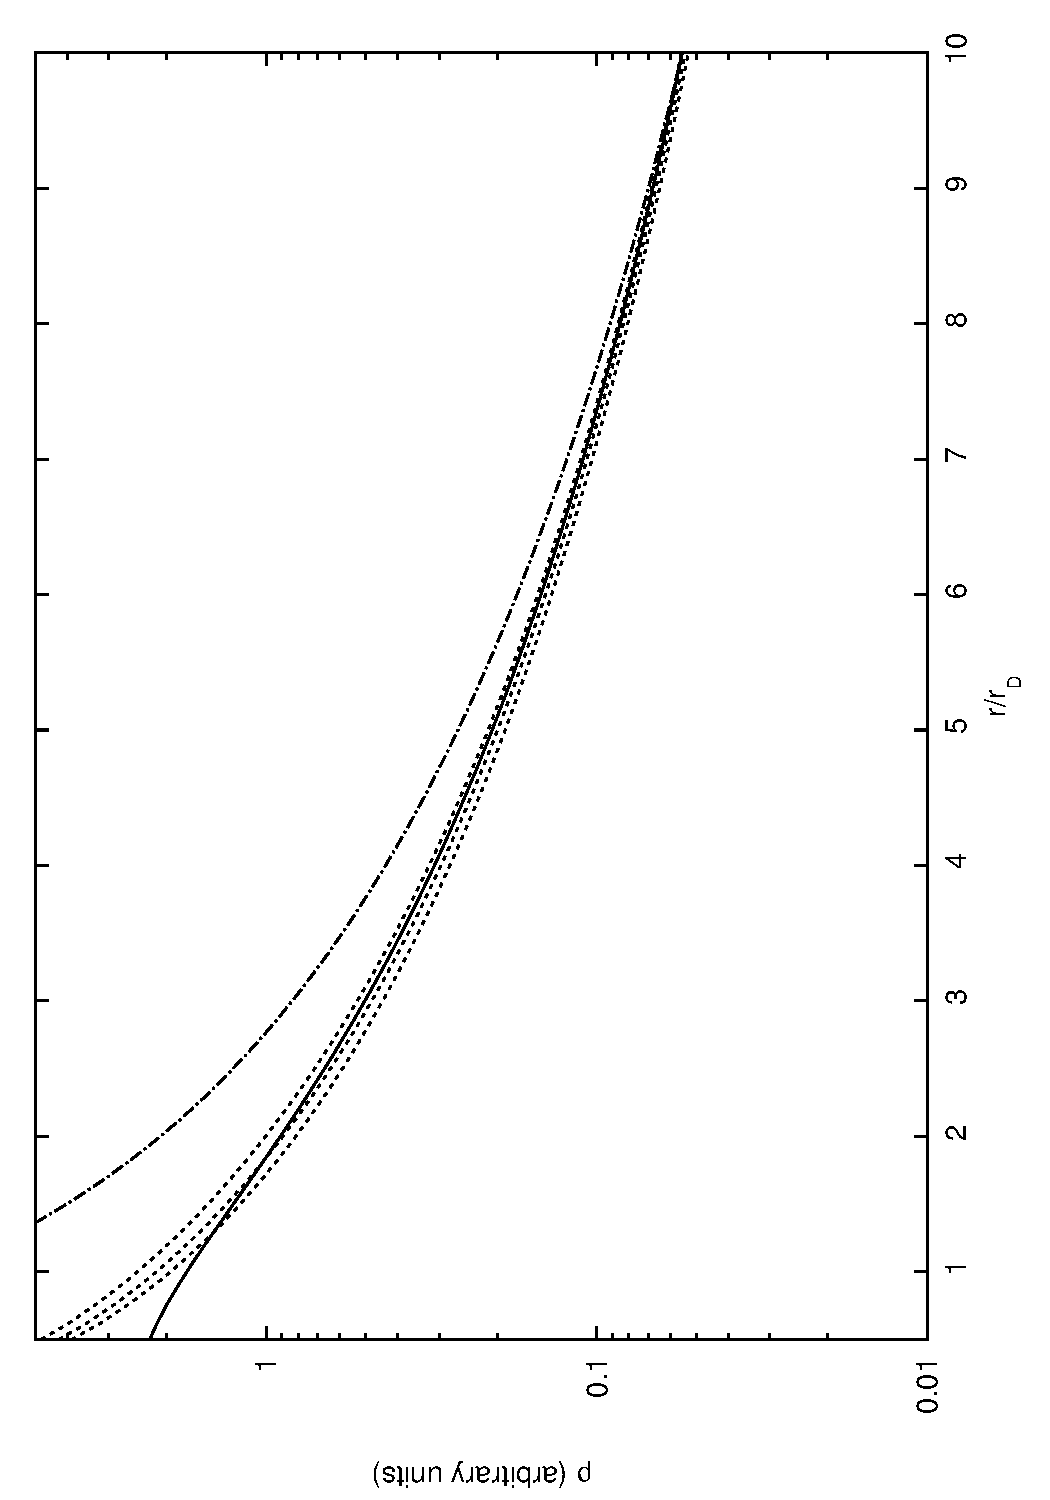
\includegraphics[scale=0.5, angle=270]{supernovater}
%        \rule{35em}{0.5pt}
    \caption{Comparison between the radial dependence of $\rho \propto f(r,\cos \phi)$, the quasi-isothermal profile given by Eq.(\ref{core}), and a cuspy profile $\rho \propto 1/r ^2$ (in arbitrary units). The dotted lines correspond to $f(r,\cos \phi)$ for (going from upper to lower line) $\phi=\pi/4,\pi/3,\pi/2$. The solid line corresponds to a cored density profile (with $r _0/r _D = 1.4$), while the dot-dashed line corresponds to the cuspy profile.}
    \label{fig:Comparison core f}
    \vskip 0.8cm
\end{figure}

Note that the dark matter density profile obtained in Eq.(\ref{core}) is cored rather than cuspy (as would be if $\rho \propto 1/r ^2$), with the cored profile arising from having smeared the supernova energy source over a finite volume. This suggests a simple explanation for the inferred existence of dark matter cores in spiral galaxies. The inability to explain the cored dark matter profile is one of the shortcomings of collisionless CDM, and is referred to as the core-cusp problem (for a review see e.g. \cite{deblok}). In addition, the scaling relation $r _0 \sim r_D$ is actually implied by measurements of high resolution rotation curves \cite{donato}:
%
\begin{eqnarray}
\log r _0 = (1.05 \pm 0.11) \log r_D + (0.33 \pm 0.04) \ .
\end{eqnarray}
%
Eq.(\ref{core}) and the scaling relation $r _0 \sim r _D$ have been derived by considering energy balance within a given galaxy. There is another piece of information we have yet to utilize. That is, demanding that the total energy input must match the total energy output for every spiral galaxy.

\subsubsection{Tully-Fisher relation}

If the system evolves to a static configuration, where the heating and cooling rates  balance, then the properties of galactic halos will be constrained. Moreover, since heating is proportional to the supernovae rate and cooling is related to the properties of dark matter, energy balance will imply a connection between the baryonic and dark matter components in spiral galaxies. The heating rate of the halo in a given spiral galaxy can be expressed as:
%
\begin{eqnarray}
\Gamma _{\text{heat}} = f _{\text{SN}}\langle E _{\text{SN}} \rangle R _{\text{SN}} \ ,
\label{tullyfisherein}
\end{eqnarray}
%
where $E _{\text{SN}}$ is the total energy output from each supernova, and $R _{\text{SN}}$ is the rate at which supernovae occur. The fraction of energy which is absorbed by the halo, $f _{\text{SN}}$, is given by:
%
\begin{eqnarray}
f _{\text{SN}} = R _{\gamma _{_D}}\langle \left (1 - e ^{-\tau} \right )\rangle \ ,
\label{fsn}
\end{eqnarray}
%
where the fraction of the total energy output in dark particles is $R _{\gamma _{_D}} \equiv E _D/E _{\text{SN}}$, $E _D$ being the amount of energy released from the supernova which is ultimately converted into the creation of dark photons. As a measure of the average optical depth, we consider dark photons propagating from the galactic centre to the edge of the galaxy (approximated as $r \rightarrow \infty$):
%
\begin{eqnarray}
\tau = \int _0 ^{\infty} dr \ \sigma _{_{DP}}n _{F_2} = \int _0 ^{\infty} dr \ \sigma _{_{DP}} \rho \kappa = \frac{\pi \sigma _{_{DP}} \kappa \rho _0r _0}{2} \ ,
\label{opticaldepth}
\end{eqnarray}
%
where we have made use of the density profile given in Eq.(\ref{core}) and related the density to the $F _2$ number density via:
%
\begin{eqnarray}
\rho = n _{F_2}(m _{F_2} + |Z'|m _{F_1}) \equiv \frac{n _{F_2}}{\kappa} \ .
\label{kappa}
\end{eqnarray}
%
Combining Eqs.(\ref{tullyfisherein}-\ref{kappa}) it follows that, in the optically thin limit, the heating rate for the halo of a given spiral galaxy is:
%
\begin{eqnarray}
\Gamma _{\text{heat}} = \frac{\pi R _{\gamma _{_D}}\sigma _{_{DP}}\kappa \langle E _{\text{SN}} \rangle}{2} \ \rho _0r _0R _{\text{SN}} \ .
\label{tullyfisherein1}
\end{eqnarray}
%

The differential cooling rate of the halo is given by Eq.(\ref{eout}). To obtain the total cooling rate Eq.(\ref{eout}) has to be integrated in the volume element. In doing so, note that the differential cooling rate depends on the parameters defining the dark matter density profile, $\rho _0$ and $r _0$, through $n _{F _1} \approx \rho \kappa (|Z'|-2)$ and $n _{F_2} = \rho \kappa$.\footnote{The relation $n _{F_1} \approx \rho \kappa (|Z'|-2)$ assumes the plasma is not fully ionized, but has the K-shell states occupied, so that dark photoionization can occur. More generally, $n _{F_1} = f\rho \kappa (|Z'|-2)$, where $f \leq 1$ accounts for partial ionization of the remaining atomic states.} Integrating Eq.(\ref{eout}) yields:
%
\begin{eqnarray}
\Gamma _{\text{cool}} = \Lambda (T)\kappa ^2 (|Z'|-2)\rho _0 ^2r _0 ^4\int _0 ^{\infty} dr' \ \frac{4\pi {r'} ^2}{({r'} ^2 + r _0 ^2) ^2} = \pi ^2\kappa ^2(|Z'|-2)\Lambda (T)\rho _0 ^2r _0 ^3 \ .
\label{tullyfishereout}
\end{eqnarray}
%
Under the assumption that the main source of dissipation is thermal dark bremsstrahlung, $\Lambda (T) \propto \sqrt{T}$ (see e.g. \cite{radiative}). The temperature $T$ is related to the rotational velocity of the galaxy far from the center, $v _{\infty}$, via Eq.(\ref{vrot}), so that $\Lambda (T) \propto \sqrt{T} \propto v _{\infty}$. The rotational velocity profile (having neglected baryonic contributions), $v _{\text{rot}}(r)$, can be related to $\rho _0$ and $r _0$ via Eq.(\ref{grhop}):
%
\begin{eqnarray}
v _{\text{rot}} ^2 = \frac{G}{r} \int _0 ^r dr' \ 4\pi {r'} ^2 \frac{\rho _0r _0 ^2}{{r'} ^2 + r _0 ^2} = 4\pi G\rho _0 r _0 ^2 \left [1 - \frac{r _0}{r}\tan ^{-1} \left ( \frac{r}{r _0} \right ) \right ] \ .
\label{vrot1}
\end{eqnarray}
%
For $r \gg r _D$, we then have:
%
\begin{eqnarray}
v _{\infty} = \left (4\pi G\rho _0r _0 ^2 \right) ^{\frac{1}{2}} \ .
\label{vrot2}
\end{eqnarray}
% 

Imposing the energy balance condition [Eq.(\ref{balance})], and hence equating $\Gamma _{\text{heat}} = \Gamma _{\text{cool}}$, with $\Gamma _{\text{heat}}$ and $\Gamma _{\text{cool}}$ given by Eqs.(\ref{tullyfisherein1},\ref{tullyfishereout}), we find:
%
\begin{eqnarray}
\Lambda (T)\rho _0 r _0 ^2 = \frac{R _{\gamma _{_D}}\sigma _{_{DP}}\langle E _{\text{SN}} \rangle}{2\pi \kappa (|Z'|-2)} \ R _{\text{SN}} \ .
\label{tullyf}
\end{eqnarray}
%
This represents a scaling relation connecting dark matter properties ($\rho _0$ and $ r_0$) with baryonic properties, such as $R _{\text{SN}}$ (and is independent of the previously obtained $r _0 \sim r _D$ relation). We show below that it is roughly equivalent to the empirical Tully-Fisher relation. Combining Eqs.(\ref{vrot2},\ref{tullyf}) and recalling that $\Lambda (T) \propto v _{\infty} \propto \left ( \rho _0 r _0 ^2 \right ) ^{\frac{1}{2}}$ results in a scaling relation connecting the supernovae rate and the asymptotic rotational velocity in a given spiral galaxy:
%
\begin{eqnarray}
R _{\text{SN}} \propto v _{\infty} ^3 \ .
\label{tullyfisher1}
\end{eqnarray}
%
Supernovae observational studies have found the relation $R _{\text{SN}} \propto \left ( L _B \right ) ^{0.73}$ \cite{wli}, where $L _B$ is the galaxy $B$-band luminosity. Combining this relation with that in Eq.(\ref{tullyfisher1}) yields:
%
\begin{eqnarray}
L _B \propto v _{\infty} ^4 \ .
\label{tullyfisher}
\end{eqnarray}
%
Eq.(\ref{tullyfisher}) is one of the forms of the Tully-Fisher relation (see e.g. \cite{webster}), an empirical relation that is believed to hold for all spiral galaxies and used extensively as a rung on the cosmic distance ladder (see for instance \cite{maoz}). The general form of the Tully-Fisher relation is $L \propto \left ( v _{\text{rot}} \right ) ^{\alpha}$, where the power $\alpha$ depends on the luminosity band under consideration. For instance, for the $K$-band (near-infrared) $\alpha = 4.35 \pm 0.14$ is determined \cite{webster}, while for the optical $B$-band $\alpha = 3.91 \pm 0.13$ is found \cite{webster}. The Tully-Fisher relation is currently unexplained, although it suggests a deep connection between the baryonic and dark matter components of spiral galaxies. Our model seems to supply such a connection via the nontrivial dissipative dynamics: the Tully-Fisher relation is the energy balance condition, Eq.(\ref{balance}), where $\Gamma _{\text{heat}}$ arises from supernovae heating and $\Gamma _{\text{cool}}$ from dissipative dynamics.\footnote{It is worth mentioning that a third relation, not independent from the other two ($r _0 \propto r _D$ and $L _B \propto v _{\infty} ^4 \propto \rho _0 ^2r _0 ^4$), can be obtained. Observational studies have shown that $m _D \propto \left ( L _B \right ) ^{1.3}$ \cite{shankar} and $r_D \propto \left ( m _D \right ) ^{0.38}$ \cite{saluccird}. Combining these relations yields $\rho _0 r _0 \approx {\rm constant}$ (which is observed to hold in spiral galaxies \cite{kormendy}).} This scenario is expected to hold within irregular galaxies as well, since these galaxies have ongoing star formation like spirals.

\subsubsection{Elliptical galaxies: the Faber-Jackson relation}

The dynamical halo model, with heating powered by kinetic mixing induced processes in the core of ordinary supernovae balancing the energy loss due to dissipative processes in the halo, seems to be
viable for galaxies with ongoing star formation: that is, spiral and irregular galaxies. This picture cannot be directly applied to elliptical galaxies as these galaxies are devoid of baryonic gas and exhibit suppressed star formation. It is possible that ellipticals could have evolved from spirals. In particular, spirals may have a final evolutionary stage where they have exhausted their baryonic gas to the point where the ordinary supernova rate is insufficient to support the dark halo from collapse.

Consider the limiting case where $t _{\text{cool}} \ll t _{\text{ff}}$, with $t _{\text{cool}}$ and $t _{\text{ff}}$ being the cooling and free-fall timescales respectively. In this limit, the dark halo can cool and potentially fragment into dark stars. Imagine a point in time where the heating suddenly stops and the halo cools but does not have time yet to collapse (consistently with $t _{\text{cool}} \ll t _{\text{ff}}$). The total energy at this time can be approximated as just the gravitational potential energy, and is given by:
%
\begin{eqnarray}
U _i = -\int _0 ^R dr \ 4\pi r^2 \frac{GM_r}{r}\rho (r) \ ,
\label{ui}
\end{eqnarray}
%
where the mass enclosed within a radius $r$ is:
%
\begin{eqnarray}
M_r = \int _0 ^r dr' \ 4\pi {r'} ^2\rho (r') \simeq 4\pi \rho _0r _0 ^2 r \ .
\end{eqnarray}
%
In evaluating $M_r$ above, we have used of the density profile given by Eq.(\ref{core}).  In the limit where $t _{\text{cool}} \ll t _{\text{ff}}$, this should be a good approximation, as the dark matter density profile has no ``time" to change. Evaluating the integral in Eq.(\ref{ui}) then gives:
%
\begin{eqnarray}
U _i = -4\pi \rho _0r _0 ^2 GM _t \ ,
\end{eqnarray}
%
where the total mass is $M _t = \int _0 ^R dr \ 4\pi r ^2 \rho \simeq 4\pi \rho _0r _0 ^2R$. 

As the system contracts, and assuming dark stars form, these stars would attain kinetic energy as they fall into the gravitational potential well. The virial theorem can then be used to relate their eventual kinetic energy, in terms of the eventual potential energy: $U _f = -2T _f$. Thus, equating this final energy with the initial energy gives:
%
\begin{eqnarray}
U _i = U _f + T _f = -T _f \ ,
\end{eqnarray}
%
By using $T _f = 3M _t\sigma _v ^2/2$, where $\sigma_v$ is the velocity dispersion of the dark stars, we find that:
\begin{eqnarray}
\sigma _v ^2 = \frac{8\pi G\rho _0r _0 ^2}{3} \ .
\end{eqnarray}
%
If, in addition, we make the assumption that the ordinary stars ``thermalize" with the dark stars, it follows that their velocity dispersion will also be approximately $\sigma _v ^2$. Given that the elliptical galaxy in the picture evolved from a spiral galaxy, the $\rho_0, r_0$ parameters obey the scaling relations derived earlier. Using the scaling relation $\rho _0r _0 \approx$ constant and $r _0 \propto r _D \propto \sqrt{L _B}$, which follows from $m _D \propto \left ( L _B \right ) ^{1.3}$ \cite{shankar} and $r_D \propto \left ( m _D \right ) ^{0.38}$ \cite{saluccird}, we obtain a relation between the $B$-band luminosity of a given elliptical galaxy and its velocity dispersion:
%
\begin{eqnarray}
L _B \propto \sigma _v ^4 \ .
\end{eqnarray}
%
Such a scaling relation, known as the Faber-Jackson relation \cite{faberjackson}, is observed to roughly hold for elliptical galaxies.

This picture of elliptical galaxies might help explain some of their distinctive properties. In particular, if the dark stars produce dark supernovae then kinetic mixing induced processes in the core of these dark supernovae can generate a large flux of ionizing ordinary photons, which can heat ordinary matter, thereby potentially explaining why elliptical galaxies are observed to be devoid of baryonic gas.

\subsection{Consistency conditions and energy balance}

The assumption that the system evolves to a static configuration has allowed us to establish a connection between the baryonic and dark matter components in spiral galaxies, in the form of scaling relations which are consistent with observations. We now wish to understand how this energy balance argument can constrain the 5-dimensional parameter space of our dark matter model. This requires a more quantitative understanding of the exact heating and cooling mechanisms.

As previously discussed, thermal dark bremsstrahlung of $F _1$ off $F _2$ is assumed to be the dominant dissipation avenue. The energy lost per unit time per unit volume due to this process is given in e.g. \cite{radiative}:
%
\begin{eqnarray}
\frac{d\Gamma _{\text{cool}}}{dV} = \frac{16 {\alpha '} ^3 (2\pi T) ^{\frac{1}{2}}}{(3 m _{F_1} ) ^{\frac{3}{2}}} {Z '} ^2 n _{F_1} n _{F_2} \overline{g} _B \ ,
\label{bremsstrahlung}
\end{eqnarray}
%
where $\overline{g} _B \simeq 1.2$ is the frequency average of the velocity-averaged Gaunt factor for thermal bremsstrahlung. 

The temperature, $T$, in Eq.(\ref{bremsstrahlung}), is related to the mean mass of the dark plasma. In the limit where $m _{F_2} \gg m _{F_1}$, and assuming neutrality of the plasma so that $n _{F_1} = (|Z'|-2)n _{F_2}$, the mean mass can be approximated by:
%
\begin{eqnarray}
\overline{m} = \frac{n _{F_1}m _{F_1} + n _{F_2}m _{F_2}}{n _{F_1} + n _{F_2}} \approx \frac{m _{F_2}}{|Z'|-1}
\label{meanmass}
\end{eqnarray}
%
Using Eqs.(\ref{vrot},\ref{core},\ref{kappa},\ref{vrot2},\ref{bremsstrahlung},\ref{meanmass}), the total cooling rate can be expressed as:
%
\begin{eqnarray}
\Gamma _{\text{cool}} = 32\pi ^3\overline{g} _B{\alpha '} ^3{Z'} ^2(|Z'|-2)\kappa ^2\sqrt{\frac{Gm _{F_2}}{27(|Z'|-1)m _{F_1} ^3}}\left ( \rho _0r _0 \right) ^{\frac{5}{2}}r _0 ^{\frac{3}{2}} \ .
\label{integratedout}
\end{eqnarray}
%

In the MDM framework it has been argued that photoionization of K-shell mirror electrons in a mirror metal component can replace the energy lost due to dissipation. This process can take place because the mirror metals in question retain their K-shell mirror electrons \cite{review}. If we assume that in our model $D ^0$ (the dark bound state), albeit being close to fully ionized, retains its K-shell $F _1$ particles, then a similar mechanism, which we call \textit{dark photoionization}, can efficiently heat the halo. The cross-section for dark photoionization, $\sigma _{_{DP}}$ can be easily obtained from that of ordinary photoionization, found in e.g. \cite{radiative}:
%
\begin{eqnarray}
\sigma _{_{DP}} = \frac{g'16\sqrt{2}\pi}{3 {m _{F_1}} ^2} {\alpha '} ^6 {|Z'|} ^5 \left ( \frac{m _{F_1}}{E _{\gamma _{_D}}} \right ) ^{\frac{7}{2}} \ ,
\label{photoionization}
\end{eqnarray}
%
where $g' = 1,2$ counts the number of K-shell $F_1$ particles present.

For the picture we have just presented to be valid, a series of consistency conditions will have to hold. We will now proceed to discuss what these conditions are and how they constrain the available parameter space for our model.

\subsubsection{Cooling timescale}

The dynamical halo picture, governed by a balance between heating and cooling rates, could only hold provided the cooling timescale is much less than the Hubble time. This requirement constrains the available parameter space and, as one can see from Eq.(\ref{integratedout}), will set an upper bound on the mass of $F_2$ [recall $\kappa ^{-1} = (m _{F_2} + |Z'|m _{F_1}$)]. If $n _T$ is the total number density of dark particles, the cooling timescale is given by:
%
\begin{eqnarray}
t _{\text{cool}} \approx \frac{\frac{3}{2}n _TT}{\Lambda (T)n _{F_1}n _{F_2}} \approx \frac{3T}{2\Lambda (T)n _{F_2}} \ ,
\label{cooling}
\end{eqnarray}
%
where we have approximated $n _T \approx n _{F_1}$. Making use of Eqs.(\ref{vrot},\ref{kappa},\ref{bremsstrahlung},\ref{meanmass}), we can write:
%
\begin{eqnarray}
t _{\text{cool}} \approx \frac{9\sqrt{3}}{64\overline{g} _B\sqrt{\pi}}\sqrt{\frac{m _{F_2}m _{F_1} ^3}{|Z'|-1}}\frac{v _{\text{rot}}}{\kappa \rho {\alpha '} ^3{Z'} ^2} \ .
\end{eqnarray}
%
Observe that the cooling timescale can be defined locally, i.e. $t _{\text{cool}}(r)$, through the dependence on $\rho (r)$. Less dense regions cool more slowly, so the most stringent limit occurs where $\rho (r)$ is lowest. Of course we have little knowledge about halo properties far from the galactic center. As a rough limit, we shall require  $t _{\text{cool}}(r) \lesssim$ few billion years, for $r \lesssim 3.2 r _D \sim 2 r _0$ (3.2 $r _D$ is the optical radius where most of the baryons reside, defined in e.g. \cite{optical}). Note that the most stringent limits occur for the largest spiral galaxies, where $\rho (r=2r _0) \approx \rho _0/5$ and $v _{\text{rot}} \approx 300 \ \rm km/s$. Here we have taken the typical values (for large spiral galaxies) $\rho _0r _0 \simeq 100 \ \rm M _{\astrosun}/pc ^2$ and $r _0 \simeq 20 \ \rm kpc$ and hence $\rho _0/5 \simeq 10 ^{-3} \ {\rm M _{\astrosun}/pc ^3}$. In this case, the requirement $t _{\text{cool}} (r=2r _0) \lesssim$ few billion years gives the upper limit on the mass of $F_2$:
%
\begin{eqnarray}
m _{F_2} \lesssim 200 \left ( \frac{\rm MeV}{m _{F_1}} \right )\left ( \frac{\alpha '}{10 ^{-2}} \right ) ^2\left ( \frac{|Z'|}{10} \right ) ^{\frac{5}{3}} \ \rm GeV \ .
\label{mf2cool}
\end{eqnarray}
%

\subsubsection{Ionization state of the halo}

The scenario described earlier assumed that the halo is ionized but the dark bound state, $D ^0$, retains its K-shell $F_1$ particles. The former requirement allows for efficient cooling via dark bremsstrahlung, while the latter is a necessary condition for dark photoionization to take place. Here we require such a picture to hold for all spiral galaxies, regardless of size. Were this not the case, one would expect significant observational differences in moving along the spectrum of spiral galaxies, depending on whether or not their dark plasma is ionized or $D ^0$ retains its K-shell $F_1$ particles. Hence we require the temperature of the halo, given in Eq.(\ref{vrot}), to be high enough to ensure that $D ^0 $ is ionized (at least one free $F_1$ particle per bound state), while being low enough as to allow the K-shell $F_1$ particles be retained. 

By comparing the appropriate ionization and capture cross-sections, in Appendix A we estimate that, given the ionization energy ${\cal I}$, the transition from an ionized to a neutral halo occurs at a temperature $T = {\cal I}/\xi$, where $\xi \approx 7-28$. Of course, in the process of obtaining a conservative lower bound on the mass of the $F_2$ particle, we are interested in the maximum value $\xi$ can assume, that is, $\xi _{\max} \approx 28$. Similarly, to obtain a conservative upper bound on $m _{F_2}$, we are interested in the minimum value $\xi$ can assume in relation to the process of K-shell photoionization. In Appendix A we estimate that $\xi _{\min} \approx \min [1/({\alpha '} ^3{Z'} ^4),1]$, and hence, denoting by ${\cal J}$ the relevant ionization energy, we obtain the rough conditions:
%
\begin{eqnarray}
T \gtrsim \frac{{\cal I}}{\xi _{\max}} \implies \frac{m _{F_2}}{\rm GeV} & \gtrsim & \left (\frac{|Z'|}{10} \right )\left (\frac{\alpha '}{10 ^{-2}} \right ) ^2\left ( \frac{m _{F_1}}{\rm MeV} \right )\left ( \frac{50 \ {\rm km/s}}{v _{\text{rot}}} \right ) ^2 \ , \nonumber \\
T \lesssim \frac{{\cal J}}{\xi _{\min}} \implies \frac{m _{F_2}}{\rm GeV} & \lesssim & 100 \left ( \frac{|Z'|}{10} \right ) ^3\left (\frac{\alpha '}{10 ^{-2}} \right ) ^2\left ( \frac{m _{F_1}}{\rm MeV} \right )\left ( \frac{300 \ {\rm km/s}}{v _{\text{rot}}} \right ) ^2g(\alpha ',Z') \ ,
\label{mf2ij}
\end{eqnarray}
%
where $g(\alpha ',Z') \equiv \max({\alpha '} ^3{Z'} ^4,1)$. Clearly the most stringent lower bound on $m _{F_2}$ arises from the smallest spiral/irregular galaxies, with $v _{\text{rot}} \approx 50 \ \rm km/s$, while the most stringent upper bound comes from the biggest spiral galaxies, for which $v _{\text{rot}} \approx 300 \ \rm km/s$, and thus:
%
\begin{eqnarray}
\left (\frac{|Z'|}{10} \right )\left (\frac{\alpha '}{10 ^{-2}} \right ) ^2\left ( \frac{m _{F_1}}{\rm MeV} \right ) \lesssim \frac{m _{F_2}}{{\rm GeV}} \lesssim 100 \left ( \frac{|Z'|}{10} \right ) ^3\left (\frac{\alpha '}{10 ^{-2}} \right ) ^2\left ( \frac{m _{F_1}}{\rm MeV} \right )g(\alpha ',Z')
\label{mf2bounds}
\end{eqnarray}
%
In addition, we have to require that the upper bound on $m _{F_2}$ [Eq.(\ref{mf2cool})] be greater than the respective lower bound [Eqs.(\ref{mf2ij})]. Doing so yields:
%
\begin{eqnarray}
|Z'| \gtrsim 4 \left ( \frac{m _{F_1}}{10 \ \rm MeV} \right ) ^3 \ .
\label{boundz}
\end{eqnarray}
%

It is conceivable that the ionization physics sets the physical scale of spiral/irregular galaxies (i.e. sets either or both $v _{\text{rot}} ^{\max}$, $v _{\text{rot}} ^{\min}$), which means that either or both the limits in Eq.(\ref{mf2bounds}) are equalities. Equating the two bounds in Eq.(\ref{mf2bounds}) we obtain that this limiting situation occurs for $|Z'| \sim 1$.

\subsubsection{Energy balance}

We now turn to the energy balance condition, $\Gamma _{\text{heat}} = \Gamma _{\text{cool}}$ [Eq.(\ref{balance})] As previously discussed, we have assumed that the galactic system evolves such that this condition is currently satisfied for spiral galaxies. Given the observed properties of spiral galaxies, we can use this condition to constrain the fundamental parameters of our model.

The cooling rate, assuming the main dissipation process being dark bremsstrahlung, is readily found [Eq.(\ref{integratedout})]. For the heating rate the situation is more complicated. Details about $\Gamma _{\text{heat}}$ require a detailed understanding of the frequency spectrum of the dark photons which, it is alleged, heat the halo. Nevertheless, we can set an upper limit on the value of this heating rate:
%
\begin{eqnarray}
\Gamma _{\text{heat}} \lesssim R _{\gamma _{_D}}R _{\text{SN}}\langle E _{\text{SN}} \rangle \min(\tau _{\max},1) \ ,
\label{gammaheat}
\end{eqnarray}
%
where $\tau _{\max}$ is the maximum value the optical depth [Eq.(\ref{opticaldepth})] can take after allowing for all possible forms of the $\gamma _{_D}$ spectrum. Eqs.(\ref{opticaldepth},\ref{photoionization}) suggest that the optical depth is maximized when $E _{\gamma _{_D}} = I'$, where $I' \approx {Z'} ^2{\alpha '} ^2m _{F_1}/2$ is the ionization energy of the relevant K-shell $F_1$ particle, hence:
%
\begin{eqnarray}
\tau _{\max} = \frac{256\pi ^2}{3}\frac{\rho _0r _0}{m _{F_1} ^2m _{F_2}\alpha '{Z'} ^2} \ .
\label{taumax}
\end{eqnarray}
%
Assuming the nominal value $\rho _0r _0 \approx 100 \ M _{\astrosun}/{\rm pc ^2} \simeq 4.6 \times 10 ^{-6} \ {\rm GeV ^3}$ and taking the upper bound on $m _{F_2}$ given in Eq.(\ref{mf2bounds}), we get:
%
\begin{eqnarray}
\tau _{\max} \gtrsim 40 \left ( \frac{\rm MeV}{m _{F_1}} \right ) ^3\left ( \frac{10 ^{-2}}{\alpha '} \right ) ^3\left ( \frac{10}{|Z'|} \right ) ^5\frac{1}{g(\alpha ',Z')} \ .
\label{tau}
\end{eqnarray}
%
Eq.(\ref{tau}) suggests $\tau _{\max}\gtrsim 1$ holds for a significant fraction of parameter space.

Let us now assume parameters where $\tau _{\max} \gtrsim 1$ and evaluate an upper limit for $\Gamma _{\text{heat}}$ (note that even with parameters where $\tau _{\max} \lesssim 1$, the derived limit will be still valid, given that $\min (\tau _{\max},1) \leq 1$). For $\epsilon \lesssim 10 ^{-9}$, $R _{\gamma _{_D}} \propto \epsilon ^2$, while for $\epsilon \gtrsim 10 ^{-9}$, $R _{\gamma _{_D}}$ actually saturates at $\sim 1/2$. By inserting numbers into Eq.(\ref{gammaheat}), we get:
%
\begin{eqnarray}
\Gamma _{\text{heat}} \lesssim \left (\frac{\epsilon}{10 ^{-9}} \right ) ^2\left (\frac{\langle E _{\text{SN}} \rangle}{3 \times 10 ^{53} \ \rm erg} \right )\left (\frac{R _{\text{SN}}}{0.03 \ \rm yr ^{-1}} \right ) 10 ^{44} \ \rm \frac{erg}{s} \ ,
\label{numberheat}
\end{eqnarray}
%
which holds for $\epsilon \lesssim 10 ^{-9}$. Similarly, inserting numbers into Eq.(\ref{integratedout}), we obtain the cooling rate for a given galaxy:
%
\begin{eqnarray}
\Gamma _{\text{cool}} \simeq \left (\frac{\alpha '}{10 ^{-2}} \right ) ^3\left (\frac{\rm MeV}{m _{F_1}} \right ) ^{\frac{3}{2}}\left ( \frac{|Z'|}{10} \right ) ^{\frac{5}{2}}\left (\frac{10 \ \rm GeV}{m _{F_2}} \right ) ^{\frac{3}{2}}\left (\frac{\rho _0r _0}{100 \ \frac{M _{\astrosun}}{\rm pc ^2}} \right ) ^{\frac{5}{2}}\left (\frac{r _0}{5 \ \rm kpc} \right ) ^{\frac{3}{2}} 10 ^{44} \ \rm \frac{erg}{s} \ .
\label{numbercool}
\end{eqnarray}
%
Comparison of Eqs.(\ref{numberheat},\ref{numbercool}) requires the following approximate relation holds:
%
\begin{eqnarray}
{\cal C}\left (\frac{10 ^{-9}}{\epsilon} \right ) ^2\left (\frac{\alpha '}{10 ^{-2}} \right ) ^3\left (\frac{\rm MeV}{m _{F_1}} \right ) ^{\frac{3}{2}}\left (\frac{|Z'|}{10} \right ) ^{\frac{5}{2}}\left (\frac{10 \ \rm GeV}{m _{F_2}} \right ) ^{\frac{3}{2}} \lesssim 1 \ ,
\label{rsn}
\end{eqnarray}
%
where:
%
\begin{eqnarray}
{\cal C} \equiv \left (\frac{\rho _0r _0}{100 \ \frac{M _{\astrosun}}{\rm pc ^2}} \right ) ^{\frac{5}{2}}\left (\frac{r _0}{5 \ \rm kpc} \right ) ^{\frac{3}{2}}\left (\frac{3 \times 10 ^{53} \ \rm erg}{\langle E _{\text{SN}} \rangle} \right )\left ( \frac{0.03 \ \rm yr ^{-1}}{R _{\text{SN}}} \right ) \ .
\label{calc}
\end{eqnarray}
%
We expect ${\cal C} \approx 1$ to hold for all spirals on account of scaling relations. In addition, Eqs.(\ref{mf2cool},\ref{rsn}) provide us with a
rough lower bound on $\epsilon$:
%
\begin{eqnarray}
\epsilon \gtrsim 10 ^{-10} \ .
\label{boundepsilon}
\end{eqnarray}
%
Note that this lower bound is consistent with the upper bounds on $\epsilon$ derived previously from early Universe cosmology.

\vskip 0.2cm

\section{Summary of the bounds on the model}

\vskip 0.1cm

Having studied the early Universe cosmology and galactic structure implications of the model, we can now make use of our analyses to constrain the 5-dimensional parameter space in question. We start by looking at the kinetic mixing parameter, $\epsilon$. The validity of our picture of galaxy structure requires core-collapse supernovae to produce a considerable energy output in light dark particles (specifically, $F_1\overline{F}_1$ pairs initially) via kinetic mixing induced processes. We have found that $\epsilon \gtrsim 10 ^{-10}$ is required for the energy output to successfully heat the halo [Eq.(\ref{boundepsilon})]. An upper bound on $\epsilon$ was derived in Section 3 from $\delta N _{\text{eff}}$[CMB] and $\delta N _{\text{eff}}$[BBN] constraints (Figure \ref{fig:Comparison bbn cmb}), which indicate $\epsilon \lesssim 5 \times 10 ^{-8}$.

As discussed in Section 2, $m _{F_1}$ is required to be bounded above by about 100 MeV, otherwise $F _1\overline{F} _1$ pair production becomes exponentially (Boltzmann) suppressed in the core of core-collapse supernovae, where the maximum temperature which can be reached is of about 30 MeV. A lower limit of around $m _{F_1} \gtrsim 0.01 \ \rm MeV$ arises from White Dwarf cooling  and Red Giants helium flash considerations \cite{updated}.

A constraint on the dark recombination temperature (so that dark acoustic oscillations do not modify the early growth of LSS) also provided a useful constraint on parameters. This constraint, Eq.(\ref{boundse}), together with the above limits on $m _{F_1}$, $\epsilon$, suggest a lower bound: $\alpha ' \gtrsim 10 ^{-4}$. Further, our analysis implicitly assumed that perturbation theory could reliably be used to calculate cross-sections, ionization energies, and so forth, which is only valid if $\alpha '$ is sufficiently small: $\alpha ' \lesssim 10 ^{-1}$.

Constraints on $m _{F_2}$ were derived from galactic structure considerations in Section 5. There it was shown that a successful picture of spiral and irregular galaxies could be achieved within this two-component hidden sector model provided $m _{F_2}$ satisfies the constraints given by Eqs.(\ref{mf2cool},\ref{mf2bounds},\ref{rsn}).

%\newpage

Below, we summarize the bounds obtained in this work:

\begin{eqnarray}
\begin{cases}
\epsilon \lesssim \min \left [3.5 \times 10 ^{-9} \left ( \frac{{\cal M}}{m _e} \right ) ^{\frac{1}{2}} \ , \ 10 ^{-8} \left ( \frac{\alpha '}{\alpha} \right ) ^4 \left ( \frac{m _{F_1}}{\rm MeV} \right ) ^2 \left ( \frac{{\cal M}}{m _e} \right ) ^{\frac{1}{2}} \right ] \ , \\
\epsilon \gtrsim 10 ^{-10} \ , \\
0.01 \ {\rm MeV} \lesssim m _{F_1} \lesssim 100 \ {\rm MeV} \ , \\
m _{F_2} \gtrsim \left (\frac{|Z'|}{10} \right )\left (\frac{\alpha '}{10 ^{-2}} \right ) ^2\left ( \frac{m _{F_1}}{\rm MeV} \right ) \ {\rm GeV} \ , \\
m _{F_2} \lesssim \min \left [200 \left ( \frac{\rm MeV}{m _{F_1}} \right )\left ( \frac{\alpha '}{10 ^{-2}} \right ) ^2\left ( \frac{|Z'|}{10} \right ) ^{\frac{5}{3}} \ , \ 100 \left ( \frac{|Z'|}{10} \right ) ^3\left (\frac{\alpha '}{10 ^{-2}} \right ) ^2\left ( \frac{m _{F_1}}{\rm MeV} \right )g(\alpha ',Z') \right ] \ {\rm GeV} , \\
10 ^{-4} \lesssim \alpha ' \lesssim 10 ^{-1} , \\
|Z'| \gtrsim \max \left [ 3, 4 \left ( \frac{m _{F_1}}{10 \ \rm MeV} \right ) ^3 \right ] \ ,
\end{cases}
\label{boundsinterrelated}
\end{eqnarray}
%
where ${\cal M} \equiv \max ( m _e, m _{F_1} )$ and $g (\alpha ',Z') \equiv \max ({\alpha '} ^3{Z'} ^4,1)$ [$m _e = 0.511 \ {\rm MeV}$ is the electron mass].

There is a finite, but certainly restricted, region of parameter space consistent with all of the above constraints. For example, if we fix $m _{F_1} = 1 \ \rm  MeV$, $\alpha ' = 10 ^{-2}, |Z'|=10$, the above constraints are all satisfied for $10 ^{-10} \lesssim \epsilon \lesssim 5 \times 10 ^{-9}$ and $1 \ {\rm GeV} \lesssim m _{F_2} \lesssim 100 \ {\rm GeV}$.

%\begin{table}[ht] 
%\caption{\textbf{Bounds on parameters of model}}
%\centering
%\footnotesize
%\begin{tabular}{c c c c}
%Parameter & Cosmology & Galaxy structure & Combined \\ [0.5ex]
%\hline
%$\epsilon$ & $\epsilon \lesssim 5 \times 10 ^{-8}$ & $\epsilon \gtrsim 2 \times 10 ^{-10}$ & $2 \times 10 ^{-10} \lesssim \epsilon \lesssim 5 \times 10 ^{-8}$ \\
%$|Z ^{'}|$ & & $|Z ^{'}| \gtrsim 2$ & $|Z ^{'}| \gtrsim 2$ \\ 
%$m _{F_1}$ & $m _{F_1} \gtrsim 0.1 \ {\rm MeV}$ & $m _{F_1} \lesssim 100 \ {\rm MeV}$ & $0.1 \ {\rm MeV} \lesssim m _{F_1} \lesssim 100 \ {\rm MeV}$  \\ 
%$m _{F_2}$ & $m _{F_2} \lesssim 10 \ {\rm TeV}$ & $m _{F_2} \gtrsim 10 \ {\rm MeV}$ & $10 \ {\rm MeV} \lesssim m _{F_2} \lesssim 10 \ {\rm TeV}$ \\ 
%$\alpha ^{'}$ & $5 \times 10 ^{-4} \lesssim \alpha ^{'} \lesssim 10 ^{-1}$ & & $5 \times 10 ^{-4} \lesssim \alpha ^{'} \lesssim 10 ^{-1}$ \\ [1ex]
%\hline
%\end{tabular} 
%\label{table:bounddd}
%\end{table}

\section{Concluding remarks}

Dark matter can be accomodated without modifying known Standard Model physics by hypothesizing the existence of a hidden sector. That is, an additional sector containing particles and forces which interact with the known Standard Model particle content predominantly via gravity. We have considered a hidden sector containing two stable particles charged under an unbroken $U(1) ^{'}$ gauge symmetry, hence featuring dissipative interactions. The associated massless gauge field, the dark photon, can interact via kinetic mixing with the ordinary photon. Our analysis indicates that such an interaction, of strength $\epsilon \sim 10^{-9}$, is required in order to explain galactic structure. We calculated the effect of this new physics on BBN and its contribution to the relativistic energy density at Hydrogen recombination. Subsequently we examined the process of dark recombination, during which neutral dark states are formed, which is important for LSS formation. We then analyzed the phenomenology of our model in the context of galactic structure, and found that it can reproduce several observed features of spiral and irregular galaxies, including the cored density profile and the Tully-Fisher relation. We have also shown how the same framework could explain some peculiar features of elliptical galaxies, which we have argued might represent the final evolutionary stage of spiral galaxies.

The above considerations constrain the five Lagrangian parameters of our model, as summarized in Eqs.(\ref{boundsinterrelated}). Note, in particular, that the kinetic mixing coupling, $\epsilon$, is constrained to lie within the range $10 ^{-10} \lesssim \epsilon \lesssim 5 \times 10 ^{-8}$. A correct simultaneous explanation of both early Universe cosmology and galactic structure typically requires one fermion, $F_1$, to be in the MeV range (or just below) and the other to be heavier, in the GeV (or possibly TeV) range. 

The allowed mass range of the two fermions means they can be, at least in principle, detected in direct detection experiments. Two types of interactions are of of particular interest in this context: $F_1$-electron scattering and $F_2$-nuclei scattering. The self-interacting nature of our model allows for $F_1$ and $F_2$ particles to accumulate in the Earth, giving rise to a unique signature: a diurnal modulation in the interaction rate. Such an effect is expected to be particularly evident for experiments located in the Southern hemisphere, giving rise to suppressions in the interaction rate which could be as large as 100\% \cite{mine}.

Although an explanation of the DAMA annual modulation signal \cite{dama1} in terms of nuclear recoils appears disfavored given the null results of the other experiments, recent work (in the context of MDM) has shown that it might be possible to explain it in terms of dark matter scattering off electrons if the mass of the dark matter particle is in the MeV range \cite{electronscattering}. Within the framework of our two-component model, a similar explanation seems possible, that is, the observed annual modulation signal in the DAMA experiment might be due to $F_1$-electron scattering.

Hidden sector dark matter models can be quite appealing from a theoretical point of view, and, as we have shown, can provide a satisfactory explanation for dark matter phenomena on both large and small scales. In our study we have constrained the parameter space of a particularly simple two component hidden sector model, and have indicated potential ways of testing such a model in the context of direct detection experiments.

%\newpage

\section*{Appendix A}

We estimate the quantity $\xi$ in Section 5.2.2. Recall, $\xi$ is defined in terms of the transition temperature between two states, at the relevant ionization energy $I'$, $T = I'/\xi$. Consider, for instance, the process relevant for $D ^0$ ionization, with cross-section $\sigma _I$:
%
\begin{eqnarray}
F_1 + D ^0 \rightarrow D ^+ + F_1 + F_1 \ ,
\label{ionziationd}
\end{eqnarray}
%
which is opposed by the corresponding capture process, with cross-section $\sigma _C$:
%
\begin{eqnarray}
F_1 + D ^+ \rightarrow D ^0 + \gamma _{_D} \ .
\label{captured}
\end{eqnarray}
%
The number density of $D ^+$ is governed by the following rate equation:
%
\begin{eqnarray}
\frac{dn _{D ^+}}{dt} = n _{F_1}n _{D ^0}\langle \sigma _Iv _{F_1}\rangle - n _{F_1}n _{D ^+}\langle \sigma _Cv _{F_1}\rangle \ .
\label{ratedp}
\end{eqnarray}
%
It follows that in a steady-state situation $n _{D ^+}/n _{D ^0}=\langle \sigma _Iv _{F_1} \rangle/\langle \sigma _Cv _{F_1} \rangle$, and hence we compare the relevant thermally averaged ionization and capture cross-sections:
%
\begin{eqnarray}
\langle \sigma _Iv _{F_1} \rangle &=& \sqrt{\frac{1}{m _{F_1}\pi}}\left (\frac{2}{T}\right ) ^{\frac{3}{2}}\int _{I'} ^{\infty} dE _{F_1}E _{F_1}e ^{-\frac{E _{F_1}}{T}}\sigma _I \ , \nonumber \\
\langle \sigma _Cv _{F_1} \rangle &=& \sqrt{\frac{1}{m _{F_1}\pi}}\left (\frac{2}{T}\right ) ^{\frac{3}{2}}\int _0 ^{\infty} dE _{F_1}E _{F_1}e ^{-\frac{E _{F_1}}{T}}\sigma _C \ .
\label{sigivsigcv}
\end{eqnarray}
%
The ionization and capture cross-sections are given in \cite{lotz,kramers} and are roughly:\footnote{The following expressions assumes the $F_1$ particles are non-relativistic, that is, $T \lesssim m _{F_1}$. If we demand that the non-relativistic approximation is valid for all spirals ($v _{\text{rot}} \lesssim 300 \ \rm km/s$), then we require $m _{F_2}/m _{F_1} \lesssim 10 ^6(|Z'|-1)$.}
%
\begin{eqnarray}
\sigma _I & \sim & \frac{{\alpha '} ^2}{E_{F_1}I'} \ , \nonumber \\
\sigma _C & \sim & \frac{{\alpha '} ^5{Z'} ^4}{E _{F_1}(E _{F_1} + I')} \ .
\end{eqnarray}
%
The relevant transition will occur when the quantity $\langle \sigma _Iv _{F_1} \rangle / \langle \sigma _Cv _{F_1} \rangle$ is of order 1, that is:
%
\begin{eqnarray}
\frac{\langle \sigma _Iv _{F_1} \rangle}{\langle \sigma _Cv _{F_1} \rangle} \sim \frac{I'+T}{I'}\frac{e ^{-\frac{I'}{T}}}{{\alpha '} ^3{Z'} ^4} \sim 1 \ ,
\end{eqnarray}
%
and hence when:
%
\begin{eqnarray}
\left ( 1+\frac{1}{\xi} \right ) e ^{-\xi} \sim {\alpha '} ^3{Z'} ^4 \ ,
\label{xiexi}
\end{eqnarray}
%
where $\xi \equiv I/T$.

For the process of $D ^0$ ionization, we can safely take $|Z'| \approx 1$. Solving Eq.(\ref{xiexi}) shows that a value of $\xi \sim 7-28$ is the solution within the allowed range of parameter space ($10 ^{-4} \lesssim \alpha ' \lesssim 10 ^{-1}$). In Section 5.2.2, Eqs.(\ref{mf2ij}), we obtain the most conservative lower bound on the mass of $F_2$ when $\xi = \xi _{\max} \approx 28$.

When analyzing the process of K-shell dark photoionization, Eqs.(\ref{mf2ij}), we obtain the most conservative upper bound on the mass of $F_2$ when $\xi$ assumes its lowest possible value. In this case we find that, to a reasonable approximation, $\xi _{\min} \approx \min [1/({\alpha '} ^3{Z'} ^4),1]$.

\section*{Appendix B}

In the paper we assumed that the dark photons arising from kinetic mixing induced processes in the core of ordinary supernovae heat the halo via a dark photoionization process. In principle, one could consider dark Thomson scattering ($\gamma _{_D}F_1 \rightarrow \gamma _{_D}F_1$, where $F_1$ denotes a free $F_1$ particle) as an equally viable heating mechanism. However, we will show below that this is not expected to be the case for the parameter space of interest.

The optical depth for dark Thomson scattering, considering a dark photon propagating from the center of the galaxy to infinity, is given by:
%
\begin{eqnarray}
\tau = \int _0 ^{\infty} dr \ \sigma _{_{DT}}n _{F_1} = \int _0 ^{\infty} dr \ \sigma _{_{DT}}\rho \kappa (|Z'|-2) = \frac{4\pi ^2{\alpha '} ^2\kappa(|Z'|-2)\rho _0r _0}{3m _{F_1} ^2} \ ,
\label{opticaldepthdark}
\end{eqnarray}
%
where we have related the free $F_1$ number density to the density profile via the relation $n _{F_1} \approx \rho \kappa (|Z'|-2)$ and made use of the expression for the dark Thomson scattering cross-section $\sigma _T = 8\pi{\alpha '} ^2/(3m _{F_1} ^2)$.

Assuming the spectrum of dark photons that heat the halo has energy spectrum that peaks well below the electron mass, kinematic considerations dictate that dark Thomson scattering can only efficiently impart energy to the scattered $F_1$ particles provided that $\tau \gg 1$ (i.e. the dark photon becomes trapped within the galaxy), and hence if:
%
\begin{eqnarray}
m _{F_2} \ll \frac{4\pi ^2\rho _0r _0}{3}\frac{{\alpha '} ^2|Z'|}{m _{F_1} ^2} \ .
\label{mf2thomson}
\end{eqnarray}
%
Here we have used $\kappa \approx 1/m _{F_2}$ [from Eq.(\ref{kappa})]. Recall, the basic requirement that the halo be ionized gave a lower bound on $m _{F_2}$ [Eqs.(\ref{mf2ij})]. Requiring that the above upper bound on $m _{F_2}$ [Eq.(\ref{mf2thomson})] be greater than the lower bound found in Eqs.(\ref{mf2ij}), we find:
%
\begin{eqnarray}
m _{F_1} ^3 \ll \frac{4\pi ^2\rho _0r _0v _{\text{rot}} ^2\xi _{\max}}{3} \ .
\label{mf1thomson}
\end{eqnarray}
%
Eq.(\ref{mf1thomson}) reduces to:
%
\begin{eqnarray}
\frac{m _{F_1}}{{\rm MeV}} \ll \left ( \frac{\rho _0r _0}{100 \ \frac{M _{\astrosun}}{{\rm pc ^2}}} \right ) ^{\frac{1}{3}}\left ( \frac{v _{\text{rot}}}{300 \ \rm km/s} \right )^{\frac{2}{3}} \ .
\end{eqnarray}
%
This is the condition for dark Thomson scattering to be a viable heating mechanism. It follows that dark Thomson scattering is not expected to be an important heating mechanism for any spirals ($v _{\text{rot}} \lesssim 300 \ \rm km/s$) if $m _{F_1} \gtrsim 0.1 \ \rm MeV$, which is the parameter range we are focusing on.

\vskip 3 cm

\begin{flushleft}

{\Large \bf Acknowledgments}

\end{flushleft}

\vskip 0.2cm
\noindent
SV would like to thank Rachel Webster, Harry Quiney, Valter Moretti and Alexander Millar for useful discussions. SV would also like to thank Jackson Clarke and Brian Le for valuable help on the computational side of this work. RF would like to thank Alexander Spencer-Smith
for useful correspondence. This work was partly supported by the Australian Research Council and the Melbourne Graduate School of Science.

%\newpage

\begin{thebibliography}{999}

\bibitem{rubin} 
  V.~C.~Rubin and W.~K.~Ford, Jr.,
  %``Rotation of the Andromeda Nebula from a Spectroscopic Survey of Emission Regions,''
  Astrophys.\ J.\  {\bf 159}, 379 (1970);
  %%CITATION = ASJOA,159,379;%%
  V.~C.~Rubin, N.~Thonnard and W.~K.~Ford, Jr.,
%``Rotational properties of 21 SC galaxies with a large range of luminosities and radii, from NGC 4605 /R = 4kpc/ to UGC 2885 /R = 122 kpc/,''
Astrophys.\ J.\  {\bf 238}, 471 (1980).
%%CITATION = ASJOA,238,471;%%
  
  \bibitem{refregier} 
  A.~Refregier,
  %``Weak gravitational lensing by large scale structure,''
  Ann.\ Rev.\ Astron.\ Astrophys.\  {\bf 41}, 645 (2003)
  [astro-ph/0307212];
  %%CITATION = ASTRO-PH/0307212;%%
  S.~Cole {\it et al.}  [2dFGRS Collaboration],
%``The 2dF Galaxy Redshift Survey: Power-spectrum analysis of the final dataset and cosmological implications,''
  Mon.\ Not.\ Roy.\ Astron.\ Soc.\  {\bf 362}, 505 (2005) [astro-ph/0501174];
%%CITATION = ASTRO-PH/0501174;%%
W.~J.~Percival {\it et al.}  [2dFGRS Collaboration],
 %``The 2dF Galaxy Redshift Survey: The Power spectrum and the matter content of   the Universe,''
 Mon.\ Not.\ Roy.\ Astron.\ Soc.\  {\bf 327}, 1297 (2001) [astro-ph/0105252].
 %%CITATION = ASTRO-PH/0105252;%%

%  \bibitem{cole}
%  S.~Cole {\it et al.}  [2dFGRS Collaboration],
%``The 2dF Galaxy Redshift Survey: Power-spectrum analysis of the final dataset and cosmological implications,''
%  Mon.\ Not.\ Roy.\ Astron.\ Soc.\  {\bf 362}, 505 (2005) [astro-ph/0501174]
%%CITATION = ASTRO-PH/0501174;%%

% \bibitem{percival}
% W.~J.~Percival {\it et al.}  [2dFGRS Collaboration],
 %``The 2dF Galaxy Redshift Survey: The Power spectrum and the matter content of   the Universe,''
% Mon.\ Not.\ Roy.\ Astron.\ Soc.\  {\bf 327}, 1297 (2001) [astro-ph/0105252];
 %%CITATION = ASTRO-PH/0105252;%%

\bibitem{dodelson} 
  S.~Dodelson,
  {\it Modern Cosmology},
  Amsterdam, Netherlands: Academic Pr. (2003) 440 p

%\bibitem{acoustic} 
 % F.~-Y.~Cyr-Racine, R.~de Putter, A.~Raccanelli and K.~Sigurdson,
  %``Constraints on Large-Scale Dark Acoustic Oscillations from Cosmology,''
  %Phys.\ Rev.\ D {\bf 89}, 063517 (2014)
  %[arXiv:1310.3278 [astro-ph.CO]].
  %%CITATION = ARXIV:1310.3278;%%
  
%\bibitem{peccei} 
  %R.~D.~Peccei,
  %``The Strong CP problem and axions,''
  %Lect.\ Notes Phys.\  {\bf 741}, 3 (2008)
  %[hep-ph/0607268].
  %%CITATION = HEP-PH/0607268;%%

%\bibitem{darkmatterprimer} 
%  K.~Garrett and G.~Duda,
  %``Dark Matter: A Primer,''
%  Adv.\ Astron.\  {\bf 2011}, 968283 (2011)
%  [arXiv:1006.2483 [hep-ph]].
  %%CITATION = ARXIV:1006.2483;%%
  
%  \bibitem{minireview} 
%  M.~Drees and G.~Gerbier,
  %``Mini-Review of Dark Matter: 2012,''
%  arXiv:1204.2373 [hep-ph].
  %%CITATION = ARXIV:1204.2373;%%
  
  \bibitem{feng} 
  J.~L.~Feng, H.~Tu and H.~-B.~Yu,
  %``Thermal Relics in Hidden Sectors,''
  JCAP {\bf 0810}, 043 (2008)
  [arXiv:0808.2318 [hep-ph]];
  %%CITATION = ARXIV:0808.2318;%%
  J.~L.~Feng, M.~Kaplinghat, H.~Tu and H.~B.~Yu,
  %``Hidden Charged Dark Matter,''
  JCAP {\bf 0907}, 004 (2009)
  [arXiv:0905.3039 [hep-ph]].
  %%CITATION = ARXIV:0905.3039;%%  
  
  \bibitem{cline6}
   D.~E.~Kaplan, G.~Z.~Krnjaic, K.~R.~Rehermann and C.~M.~Wells,
  %``Atomic Dark Matter,''
  JCAP {\bf 1005} (2010) 021
  [arXiv:0909.0753 [hep-ph]];
  D.~E.~Kaplan, G.~Z.~Krnjaic, K.~R.~Rehermann and C.~M.~Wells,
  %``Dark Atoms: Asymmetry and Direct Detection,''
  JCAP {\bf 1110} (2011) 011
  [arXiv:1105.2073 [hep-ph]];
  %%CITATION = ARXIV:1105.2073;%%
  %%CITATION = ARXIV:0909.0753;%%
  J.~M.~Cline, Z.~Liu and W.~Xue,
  %``Millicharged Atomic Dark Matter,''
  Phys.\ Rev.\ D {\bf 85} (2012) 101302
  [arXiv:1201.4858 [hep-ph]];
  %%CITATION = ARXIV:1201.4858;%%
  F.~Y.~Cyr-Racine and K.~Sigurdson,
  %``Cosmology of atomic dark matter,''
  Phys.\ Rev.\ D {\bf 87} (2013) 10,  103515
  [arXiv:1209.5752 [astro-ph.CO]];
  %%CITATION = ARXIV:1209.5752;%%
  J.~M.~Cline, Z.~Liu, G.~Moore and W.~Xue,
  %``Composite strongly interacting dark matter,''
  arXiv:1312.3325 [hep-ph].
  %%CITATION = ARXIV:1312.3325;%%
  
  \bibitem{ringwald}
  A.~Ibarra, A.~Ringwald and C.~Weniger,
  %``Hidden gauginos of an unbroken U(1): Cosmological constraints and phenomenological prospects,''
  JCAP {\bf 0901} (2009) 003
  [arXiv:0809.3196 [hep-ph]];
  %%CITATION = ARXIV:0809.3196;%%
  S.~Andreas, M.~D.~Goodsell and A.~Ringwald,
  %``Dark Matter and Dark Forces from a Supersymmetric Hidden Sector,''
  Phys.\ Rev.\ D {\bf 87} (2013) 025007
  [arXiv:1109.2869 [hep-ph]];
  %%CITATION = ARXIV:1109.2869;%%
  S.~Andreas, M.~D.~Goodsell and A.~Ringwald,
  %``Hidden Photons in connection to Dark Matter,''
  AIP Conf.\ Proc.\  {\bf 1563} (2013) 114
  [arXiv:1306.1168 [hep-ph]];
  %%CITATION = ARXIV:1306.1168;%%
  N.~Arkani-Hamed, D.~P.~Finkbeiner, T.~R.~Slatyer and N.~Weiner,
  %``A Theory of Dark Matter,''
  Phys.\ Rev.\ D {\bf 79} (2009) 015014
  [arXiv:0810.0713 [hep-ph]].
  %%CITATION = ARXIV:0810.0713;%%
  
\bibitem{broken}
  J.~W.~Cui, H.~J.~He, L.~C.~Lu and F.~R.~Yin,
  %``Spontaneous Mirror Parity Violation, Common Origin of Matter and Dark Matter, and the LHC Signatures,''
  Phys.\ Rev.\ D {\bf 85} (2012) 096003
  [arXiv:1110.6893 [hep-ph]].
  %%CITATION = ARXIV:1110.6893;%%
  
  \bibitem{fundamentalimproper} 
  R.~Foot, H.~Lew and R.~R.~Volkas,
  %``A Model with fundamental improper space-time symmetries,''
  Phys.\ Lett.\ B {\bf 272}, 67 (1991).
  %%CITATION = PHLTA,B272,67;%%
  
  \bibitem{berezhiani}
  Z.~Berezhiani, D.~Comelli and F.~L.~Villante,
  %``The Early mirror universe: Inflation, baryogenesis, nucleosynthesis and dark matter,''
  Phys.\ Lett.\ B {\bf 503}, 362 (2001)
  [hep-ph/0008105];
  %%CITATION = HEP-PH/0008105;%%
  A.~Y.~.Ignatiev and R.~R.~Volkas,
  %``Mirror dark matter and large scale structure,''
  Phys.\ Rev.\ D {\bf 68}, 023518 (2003)
  [hep-ph/0304260];
  %%CITATION = HEP-PH/0304260;%%
  Z.~Berezhiani, P.~Ciarcelluti, D.~Comelli and F.~L.~Villante,
  %``Structure formation with mirror dark matter: CMB and LSS,''
  Int.\ J.\ Mod.\ Phys.\ D {\bf 14}, 107 (2005)
  [astro-ph/0312605];
  %%CITATION = ASTRO-PH/0312605;%%
  P.~Ciarcelluti,
  %``Cosmology of the mirror universe,''
  astro-ph/0312607.
  %%CITATION = ASTRO-PH/0312607;%%
  
  \bibitem{mirrormattertype} 
  R.~Foot,
  %``Mirror matter-type dark matter,''
  Int.\ J.\ Mod.\ Phys.\ D {\bf 13}, 2161 (2004)
  [astro-ph/0407623].
  %%CITATION = ASTRO-PH/0407623;%%
  
  \bibitem{spheroidal} 
  R.~Foot and R.~R.~Volkas,
  %``Spheroidal galactic halos and mirror dark matter,''
  Phys.\ Rev.\ D {\bf 70}, 123508 (2004)
  [astro-ph/0407522].
  %%CITATION = ASTRO-PH/0407522;%%

  \bibitem{depth4}
  R.~Foot,
  %``Galactic structure explained with dissipative mirror dark matter,''
  Phys.\ Rev.\ D {\bf 88}, 023520 (2013)
  [arXiv:1304.4717 [astro-ph.CO]];
  %%CITATION = ARXIV:1304.4717;%%
  R.~Foot,
  %``Tully-Fisher relation, galactic rotation curves and dissipative mirror dark matter,''
  arXiv:1307.1755 [astro-ph.GA];
  %%CITATION = ARXIV:1307.1755;%%
  R.~Foot,
  %``A dark matter scaling relation from mirror dark matter,''
  arXiv:1303.1727 [astro-ph.CO].
  %%CITATION = ARXIV:1303.1727;%%
  
\bibitem{dama1}
  R.~Bernabei {\it et al.},
  %``Dark matter search,''
  Riv.\ Nuovo Cim.\  {\bf 26N1} (2003) 1
  [astro-ph/0307403];
  %%CITATION = ASTRO-PH/0307403;%%
  %\cite{Bernabei:2008yi}
  R.~Bernabei {\it et al.}  [DAMA Collaboration],
  %``First results from DAMA/LIBRA and the combined results with DAMA/NaI,''
  Eur.\ Phys.\ J.\ C {\bf 56} (2008) 333
  [arXiv:0804.2741 [astro-ph]];
  %%CITATION = ARXIV:0804.2741;%%
  R.~Bernabei {\it et al.},
  %``Final model independent result of DAMA/LIBRA-phase1,''
  Eur.\ Phys.\ J.\ C {\bf 73} (2013) 2648
  [arXiv:1308.5109 [astro-ph.GA]].
  %%CITATION = ARXIV:1308.5109;%%
  
    \bibitem{cogent}
  C.~E.~Aalseth {\it et al.},
  %``Search for an Annual Modulation in a P-type Point Contact Germanium Dark Matter Detector,''
  Phys.\ Rev.\ Lett.\  {\bf 107} (2011) 141301
  [arXiv:1106.0650 [astro-ph.CO]];
  %%CITATION = ARXIV:1106.0650;%%
  C.~E.~Aalseth {\it et al.}  [CoGeNT Collaboration],
  %``Search for An Annual Modulation in Three Years of CoGeNT Dark Matter Detector Data,''
  arXiv:1401.3295 [astro-ph.CO].
  %%CITATION = ARXIV:1401.3295;%%
  
  \bibitem{dama} 
  R.~Foot,
  %``A comprehensive analysis of the dark matter direct detection experiments in the mirror dark matter framework,''
  Phys.\ Rev.\ D {\bf 82}, 095001 (2010)
  [arXiv:1008.0685 [hep-ph]];
  %%CITATION = ARXIV:1008.0685;%%
  R.~Foot,
  %``Direct detection experiments explained with mirror dark matter,''
  Phys.\ Lett.\ B {\bf 728}, 45 (2014)
  [arXiv:1305.4316 [astro-ph.CO]].
  %%CITATION = ARXIV:1305.4316;%%
  
  \bibitem{electronscattering}
  R.~Foot,
  %``Can dark matter - electron scattering explain the DAMA annual modulation signal?,''
  arXiv:1407.4213 [hep-ph].
  %%CITATION = ARXIV:1407.4213;%%  
  
  \bibitem{review}
  R.~Foot,
  %``Mirror dark matter: Cosmology, galaxy structure and direct detection,''
  Int.\ J.\ Mod.\ Phys.\ A {\bf 29}, 1430013 (2014)
  [arXiv:1401.3965 [astro-ph.CO]].
  %%CITATION = ARXIV:1401.3965;%%

\bibitem{reviewadm}
  R.~R.~Volkas,
  %``Brief Overview of Asymmetric Dark Matter,''
  Universe {\bf 1} (2013) 3,  4;
  K.~Petraki and R.~R.~Volkas,
  %``Review of asymmetric dark matter,''
  Int.\ J.\ Mod.\ Phys.\ A {\bf 28} (2013) 1330028
  [arXiv:1305.4939 [hep-ph]];
  %%CITATION = ARXIV:1305.4939;%%
  K.~M.~Zurek,
  %``Asymmetric Dark Matter: Theories, Signatures, and Constraints,''
  Phys.\ Rept.\  {\bf 537} (2014) 91
  [arXiv:1308.0338 [hep-ph]].
  %%CITATION = ARXIV:1308.0338;%%
  
\bibitem{foothe}
  R.~Foot and X.~G.~He,
  %``Comment on Z Z-prime mixing in extended gauge theories,''
  Phys.\ Lett.\ B {\bf 267} (1991) 509.
  %%CITATION = PHLTA,B267,509;%%
  
  \bibitem{holdom} 
  B.~Holdom,
  %``Two U(1)'s and Epsilon Charge Shifts,''
  Phys.\ Lett.\ B {\bf 166}, 196 (1986).
  %%CITATION = PHLTA,B166,196;%%
  
  \bibitem{hiddensector} 
  R.~Foot,
  %``Hidden sector dark matter explains the DAMA, CoGeNT, CRESST-II and CDMS/Si experiments,''
  Phys.\ Rev.\ D {\bf 88}, no. 2, 025032 (2013)
  [arXiv:1209.5602 [hep-ph]].
  %%CITATION = ARXIV:1209.5602;%%
  
  \bibitem{petrakiatomic}
  K.~Petraki, L.~Pearce and A.~Kusenko,
  %``Self-interacting asymmetric dark matter coupled to a light massive dark photon,''
  JCAP {\bf 1407} (2014) 039
  [arXiv:1403.1077 [hep-ph]].
  %%CITATION = ARXIV:1403.1077;%%
  
\bibitem{goldberghall}
  H.~Goldberg and L.~J.~Hall,
  %``A New Candidate for Dark Matter,''
  Phys.\ Lett.\ B {\bf 174} (1986) 151.
  %%CITATION = PHLTA,B174,151;%%
  
    \bibitem{dddm}
  J.~Fan, A.~Katz, L.~Randall and M.~Reece,
  %``Dark-Disk Universe,''
  Phys.\ Rev.\ Lett.\  {\bf 110} (2013) 21,  211302
  [arXiv:1303.3271 [hep-ph]];
  %%CITATION = ARXIV:1303.3271;%%
  J.~Fan, A.~Katz and J.~Shelton,
  %``Direct and indirect detection of dissipative dark matter,''
  JCAP {\bf 1406} (2014) 059
  [arXiv:1312.1336 [hep-ph]].
  %%CITATION = ARXIV:1312.1336;%%

   \bibitem{raf}
  G.~G.~Raffelt,
  ``Stars as laboratories for fundamental physics : The astrophysics of neutrinos, axions, and other weakly interacting particles,''
  Chicago, USA: Univ. Pr. (1996) 664 p.

 \bibitem{redgiants}
  M.~I.~Dobroliubov and A.~Y.~Ignatiev,
  %``Millicharged Particles,''
  Phys.\ Rev.\ Lett.\  {\bf 65} (1990) 679.
  %%CITATION = PRLTA,65,679;%%
  
  \bibitem{whitedwarfs}
  J.~Bernstein, M.~Ruderman and G.~Feinberg,
  %``Electromagnetic Properties of the neutrino,''
  Phys.\ Rev.\  {\bf 132} (1963) 1227;
  %%CITATION = PHRVA,132,1227;%%
  J.~R.~Ellis and K.~A.~Olive,
  %``Constraints on Light Particles From Stellar Evolution,''
  Nucl.\ Phys.\ B {\bf 223} (1983) 252.
  %%CITATION = NUPHA,B223,252;%%

  \bibitem{updated}
  S.~Davidson, S.~Hannestad and G.~Raffelt,
  %``Updated bounds on millicharged particles,''
  JHEP {\bf 0005} (2000) 003
  [hep-ph/0001179].
  %%CITATION = HEP-PH/0001179;%%
  
  \bibitem{bailey}
  S.~Davidson, B.~Campbell and D.~C.~Bailey,
  %``Limits on particles of small electric charge,''
  Phys.\ Rev.\ D {\bf 43} (1991) 2314.
  %%CITATION = PHRVA,D43,2314;%%
  
  \bibitem{poincare}
  R.~Foot, A.~Kobakhidze, K.~L.~McDonald and R.~R.~Volkas,
  %``Poincare Protection for a Natural Electroweak Scale,''
  Phys.\ Rev.\ D {\bf 89} (2014) 115018
  [arXiv:1310.0223 [hep-ph]],
  see also
  %%CITATION = ARXIV:1310.0223;%%
  R.~R.~Volkas, A.~J.~Davies and G.~C.~Joshi,
  %``Naturalness Of The Invisible Axion Model,''
  Phys.\ Lett.\ B {\bf 215} (1988) 133.
  %%CITATION = PHLTA,B215,133;%%
  
  \bibitem{hodges}
  E.~W.~Kolb, D.~Seckel and M.~S.~Turner,
  %``The Shadow World,''
  Nature {\bf 314} (1985) 415;
  %%CITATION = NATUA,314,415;%%
H.~M.~Hodges,
%``Mirror baryons as the dark matter,''
Phys.\ Rev.\ D {\bf 47}, 456 (1993);
%%CITATION = PHRVA,D47,456;%%
 Z.~G.~Berezhiani, A.~D.~Dolgov and R.~N.~Mohapatra,
  %``Asymmetric inflationary reheating and the nature of mirror universe,''
  Phys.\ Lett.\ B {\bf 375} (1996) 26
  [hep-ph/9511221].
  %%CITATION = HEP-PH/9511221;%%
  
  \bibitem{redondo}
  H.~Vogel and J.~Redondo,
  %``Dark Radiation constraints on minicharged particles in models with a hidden photon,''
  JCAP {\bf 1402} (2014) 029
  [arXiv:1311.2600 [hep-ph]].
  %%CITATION = ARXIV:1311.2600;%%
  
  \bibitem{predictions} 
  R.~Foot,
  %``Mirror dark matter cosmology - predictions for $N _{\text{eff}} [CMB]$ and $N _{\text{eff}} [BBN]$,''
  Phys.\ Lett.\ B {\bf 711}, 238 (2012)
  [arXiv:1111.6366 [astro-ph.CO]].
  %%CITATION = ARXIV:1111.6366;%%
  
 \bibitem{carlson}
 E.~D.~Carlson and S.~L.~Glashow,
 %``Nucleosynthesis Versus The Mirror Universe,''
 Phys.\ Lett.\ B {\bf 193}, 168 (1987).
 %%CITATION = PHLTA,B193,168;%%  
  
 \bibitem{ciarcellutiliege} 
  P.~Ciarcelluti and R.~Foot,
  %``Early Universe cosmology in the light of the mirror dark matter interpretation of the DAMA/Libra signal,''
  Phys.\ Lett.\ B {\bf 679}, 278 (2009)
  [arXiv:0809.4438 [astro-ph]].
  %%CITATION = ARXIV:0809.4438;%%
  
  \bibitem{gondologelmini} 
  P.~Gondolo and G.~Gelmini,
  %``Cosmic abundances of stable particles: Improved analysis,''
  Nucl.\ Phys.\ B {\bf 360}, 145 (1991).
  %%CITATION = NUPHA,B360,145;%%  

   \bibitem{earlyuniverse} 
  E.~W.~Kolb and M.~S.~Turner,
  {\it The Early Universe}
  Front.\ Phys.\  {\bf 69}, 1 (1990).
  %%CITATION = FRPHA,69,1;%%
  
 \bibitem{feynman} 
  R.~P.~Feynman, R.~B. Leighton and M. Sands, {\it Feynman Lectures on Physics}, Volume I (1964). 
 
  \bibitem{mangano} 
  G.~Mangano, G.~Miele, S.~Pastor, T.~Pinto, O.~Pisanti and P.~D.~Serpico,
  %``Relic neutrino decoupling including flavor oscillations,''
  Nucl.\ Phys.\ B {\bf 729}, 221 (2005)
  [hep-ph/0506164].
  %%CITATION = HEP-PH/0506164;%% 
  
  \bibitem{wmapx}
  E.~Komatsu {\it et al.}  [WMAP Collaboration],
  %``Seven-Year Wilkinson Microwave Anisotropy Probe (WMAP) Observations: Cosmological Interpretation,''
  Astrophys.\ J.\ Suppl.\  {\bf 192}, 18 (2011)
  [arXiv:1001.4538 [astro-ph.CO]].
  
  \bibitem{sptx}
   R.~Keisler {\it et al.},
%``A Measurement of the Damping Tail of the Cosmic Microwave
%Background Power Spectrum with the South Pole Telescope,''
Astrophys.\ J.\  {\bf 743}, 28 (2011) [arXiv:1105.3182].
%%CITATION = ARXIV:1105.3182;%%
  
  \bibitem{atax}
  %%CITATION = ARXIV:1001.4538;%%
  J.~Dunkley {\it et al.},
  %``The Atacama Cosmology Telescope: Cosmological Parameters from the 2008 Power Spectra,''
  Astrophys.\ J.\  {\bf 739}, 52 (2011)
  [arXiv:1009.0866 [astro-ph.CO]].
  %%CITATION = ARXIV:1009.0866;%%
 
  \bibitem{plax}
  P.~A.~R.~Ade {\it et al.}  [Planck Collaboration],
  %``Planck 2013 results. XVI. Cosmological parameters,''
  arXiv:1303.5076 [astro-ph.CO].
  %%CITATION = ARXIV:1303.5076;%%
  
  \bibitem{weinberg}
  S.~Weinberg,
  {\it Cosmology},
  Oxford, UK: Oxford Univ. Pr. (2008) 593 p.
  
  \bibitem{bernstein}
  J.~Bernstein, L.~S.~Brown and G.~Feinberg,
  %``Cosmological Helium Production Simplified,''
  Rev.\ Mod.\ Phys.\  {\bf 61} (1989) 25.
  %%CITATION = RMPHA,61,25;%%
  
  \bibitem{izotov} 
  Y.~I.~Izotov and T.~X.~Thuan,
  %``The primordial abundance of 4He: evidence for non-standard big bang nucleosynthesis,''
  Astrophys.\ J.\  {\bf 710}, L67 (2010)
  [arXiv:1001.4440 [astro-ph.CO]];
  %%CITATION = ARXIV:1001.4440;%%
  E.~Aver, K.~A.~Olive and E.~D.~Skillman,
  %``A New Approach to Systematic Uncertainties and Self-Consistency in Helium Abundance Determinations,''
  JCAP {\bf 1005}, 003 (2010)
  [arXiv:1001.5218 [astro-ph.CO]].
  %%CITATION = ARXIV:1001.5218;%%
  
  \bibitem{volkaspetraki} 
  K.~Petraki, M.~Trodden and R.~R.~Volkas,
  %``Visible and dark matter from a first-order phase transition in a baryon-symmetric universe,''
  JCAP {\bf 1202}, 044 (2012)
  [arXiv:1111.4786 [hep-ph]].
  %%CITATION = ARXIV:1111.4786;%%
  
  \bibitem{implications} 
  R.~Foot,
  %``Implications of mirror dark matter kinetic mixing for CMB anisotropies,''
  Phys.\ Lett.\ B {\bf 718}, 745 (2013)
  [arXiv:1208.6022 [astro-ph.CO]].
   %%CITATION = ARXIV:1208.6022;%%
 
\bibitem{cia}
  P.~Ciarcelluti and Q.~Wallemacq,
  %``Is dark matter made of mirror matter? Evidence from cosmological data,''
  Phys.\ Lett.\ B {\bf 729} (2014) 62
  [arXiv:1211.5354 [astro-ph.CO]].
  %%CITATION = ARXIV:1211.5354;%%
  
  \bibitem{pdg} 
  J.~Beringer {\it et al.}  [Particle Data Group Collaboration],
  %``Review of Particle Physics (RPP),''
  Phys.\ Rev.\ D {\bf 86}, 010001 (2012).
  %%CITATION = PHRVA,D86,010001;%%
  
\bibitem{silagadze}
  R.~Foot and Z.~K.~Silagadze,
  %``Supernova explosions, 511-keV photons, gamma ray bursts and mirror matter,''
  Int.\ J.\ Mod.\ Phys.\ D {\bf 14} (2005) 143
  [astro-ph/0404515].
  %%CITATION = ASTRO-PH/0404515;%%

  \bibitem{schmidt} 
  M.~Schmidt,
  %``The Rate of Star Formation,''
  Astrophys.\ J.\  {\bf 129}, 243 (1959).
  %%CITATION = ASJOA,129,243;%%
  
%  \bibitem{snaith}
% O.~N.~Snaith {\it et al.}, arXiv:1401.1835.
 
 \bibitem{radiative}
 G. ~B. ~Rybicki and A.~P. ~Lightman,
 {\it Radiative processes in astrophysics},
 Wiley, (2008).
 
\bibitem{freeman}
  K.~C.~Freeman,
  %``On the disks of spiral and SO Galaxies,''
  Astrophys.\ J.\  {\bf 160} (1970) 811.
  %%CITATION = ASJOA,160,811;%%

 \bibitem{deblok}
  W.~J.~G.~de Blok,
  %``The Core-Cusp Problem,''
  Adv.\ Astron.\  {\bf 2010} (2010) 789293
  [arXiv:0910.3538 [astro-ph.CO]].
  %%CITATION = ARXIV:0910.3538;%%
  
 \bibitem{donato}
 F.~Donato and P.~Salucci,
 %``Cores of dark matter halos correlate with disk scale lengths,''
 Mon.\ Not.\ Roy.\ Astron.\ Soc.\  {\bf 353}, L17 (2004) [astro-ph/0403206].
 %%CITATION = ASTRO-PH/0403206;%%
 
 \bibitem{wli}
W.~Li {\it et al.}, 
%``Nearby Supernova Rates from the Lick Observatory Supernova Search. 
%III. The Rate-Size Relation, and the Rates as a Function of Galaxy 
% Hubble Type and Colour,''
Mon.\ Not.\ Roy.\ Astron.\ Soc.\  {\bf 412}, 1473 (2011) [arXiv:1006.4613].
%%CITATION = ARXIV:1006.4613;%%
  
  \bibitem{webster}
 M. J. Meyer, M. A. Zwaan, R. L. Webster, S. Schneider and L. Staveley-Smith,
 Mon.\ Not.\ Roy.\ Astron.\ Soc.\  {\bf 391}, 1712 (2008).
 
 \bibitem{maoz}
  D.~Maoz,
  {\it Astrophysics in a Nutshell},
  Princeton Univ. Pr. (2007) 249 p.

\bibitem{shankar}
 F.~Shankar, A.~Lapi, P.~Salucci, G.~De Zotti and L.~Danese,
 %``New relationships between galaxy properties and host halo mass, and
 %the role of feedbacks in galaxy formation,''
 Astrophys.\ J.\  {\bf 643}, 14 (2006)
 [astro-ph/0601577].
 %%CITATION = ASTRO-PH/0601577;%%

 \bibitem{saluccird}
P.~Salucci, A.~Lapi, C.~Tonini, G.~Gentile, I.~Yegorova and U.~Klein,
%``The Universal Rotation Curve of Spiral Galaxies. 2. The Dark Matter Distribution out to the Virial Radius,''
Mon.\ Not.\ Roy.\ Astron.\ Soc.\  {\bf 378}, 41 (2007) [astro-ph/0703115].
%%CITATION = ASTRO-PH/0703115;%%

 \bibitem{kormendy}
 J.~Kormendy, K.~C.~Freeman, 2004, IAU Symposium, 220, 337

 %\cite{Faber:1976sn}
\bibitem{faberjackson}
  S.~M.~Faber and R.~E.~Jackson,
  %``Velocity dispersions and mass to light ratios for elliptical galaxies,''
  Astrophys.\ J.\  {\bf 204} (1976) 668.
  %%CITATION = ASJOA,204,668;%%
  
\bibitem{optical}
  G.~Gentile, P.~Salucci, U.~Klein and G.~L.~Granato,
  %``NGC 3741: Dark halo profile from the most extended rotation curve,''
  Mon.\ Not.\ Roy.\ Astron.\ Soc.\  {\bf 375} (2007) 199
  [astro-ph/0611355].
  %%CITATION = ASTRO-PH/0611355;%%
  
% \bibitem{madau}
% P.~Madau,
 %``The Astrophysics of Early Galaxy Formation,''
% arXiv:0706.0123 [astro-ph].
 %%CITATION = ARXIV:0706.0123;%%
  
  \bibitem{mine}
   R.~Foot, S.~Vagnozzi, work in progress.
   
   \bibitem{lotz}
W. ~Lotz, \ Z.\ Phys.\ {\bf 216}, 241 (1968).

\bibitem{kramers}
Y.~S.~Kim and R.~H.~Pratt,
%``Direct Radiative Recombination Of Electrons With Atomic Ions: Cross-sections And Rate Coefficients,''
Phys.\ Rev.\ A {\bf 27}, 2913 (1983).
%%CITATION = PHRVA,A27,2913;%%
  
% \bibitem{lux}
  %D.~S.~Akerib {\it et al.}  [LUX Collaboration],
  %``First results from the LUX dark matter experiment at the Sanford Underground Research Facility,''
  %Phys.\ Rev.\ Lett.\  {\bf 112} (2014) 091303
  %[arXiv:1310.8214 [astro-ph.CO]].
  %%CITATION = ARXIV:1310.8214;%%
  
 %\bibitem{xenon}
  %E.~Aprile {\it et al.}  [XENON100 Collaboration],
  %``Dark Matter Results from 225 Live Days of XENON100 Data,''
  %Phys.\ Rev.\ Lett.\  {\bf 109} (2012) 181301
  %[arXiv:1207.5988 [astro-ph.CO]].
  %%CITATION = ARXIV:1207.5988;%%
  
 %\bibitem{cdms}
  %R.~Agnese {\it et al.}  [SuperCDMS Collaboration],
  %``Search for Low-Mass WIMPs with SuperCDMS,''
  %Phys.\ Rev.\ Lett.\  {\bf 112} (2014) 241302
  %[arXiv:1402.7137 [hep-ex]].
  %%CITATION = ARXIV:1402.7137;%%
  
 %\bibitem{cresst}
  %G.~Angloher {\it et al.}  [ CRESST Collaboration],
  %``Results on low mass WIMPs using an upgraded CRESST-II detector,''
  %arXiv:1407.3146 [astro-ph.CO].
  %%CITATION = ARXIV:1407.3146;%%
  
 %\bibitem{cdex}
  %Q.~Yue {\it et al.}  [CDEX Collaboration],
  %``Limits on light WIMPs from the CDEX-1 experiment with a p-type point-contact germanium detector at the China Jingping Underground Laboratory,''
  %arXiv:1404.4946 [hep-ex].
  %%CITATION = ARXIV:1404.4946;%%
  
 %\bibitem{c4}
  %R.~M.~Bonicalzi {\it et al.}  [C-4 Collaboration],
  %``The C-4 Dark Matter Experiment,''
  %Nucl.\ Instrum.\ Meth.\ A {\bf 712} (2013) 27
  %[arXiv:1210.6282 [astro-ph.CO]].
  %%CITATION = ARXIV:1210.6282;%%
  
\end{thebibliography}

\end{document}

